\documentclass[12pt]{report}
\usepackage[margin=1in]{geometry} % change margins
\usepackage{graphicx} % inserting images
\usepackage{caption} % captions
\usepackage{amsmath} % for better math
\usepackage{verbatim} %used for comment blocks
\usepackage{mathtools}
\usepackage[english]{babel}
\usepackage[colorinlistoftodos]{todonotes}
\usepackage{placeins}
\usepackage[square, sort, numbers]{natbib}
\usepackage{url}
\usepackage{setspace}
\usepackage{breqn}
\usepackage{subcaption}
\usepackage{textcomp}
\usepackage{float}
\usepackage{leftidx}
\usepackage{bm}
\usepackage[titletoc,toc, title]{appendix}
\usepackage[utf8]{inputenc}
\usepackage{diagbox}
\usepackage{hyperref}
\usepackage{tcolorbox}

\usepackage{amsmath,amssymb,braket,cancel,nicefrac,physics,tensor,slashed}
\usepackage{color,empheq,enumitem,forloop,graphicx,microtype,subcaption,verbatim,wrapfig,pdfpages,titlesec}
\usepackage{array,booktabs,multicol,multirow,tabularx} 

\def\cesar#1{{\color{blue}[#1]}}
\def\anhkhoi#1{{\color{purple}[#1]}}
\def\nikr#1{{\color{red} #1}}
\def\nikb#1{{\color{magenta} (#1)}}

\tcbset{colback=blue!5!white,colframe=blue!75!black,center,halign=justify,width=0.9\textwidth,fonttitle=\bfseries}

\linespread{1.15}
\title{PHYS 102: TA Lab Manual}
\author{Nikolas Provatas (Instructor), \\ Anh-Khoi Trinh, Cesar Daniel Rodriguez Rosenblueth}

\begin{document}
\maketitle

\tableofcontents

\part{General Guidelines} \label{Sec:Intro}

\chapter{Lab Format}

\section{Introduction, Learning Objectives and Lab Structure}
Welcome to PHYS 102! The focus of these lab sessions will be to practice critical thinking about data collected from experiments, a skill that can be applied in many other STEM fields and in your own personal lives. You will also learn how to acquire and analyse data quantitatively in experiments pertaining to electromagnetism experiments. \\

\noindent \large \textbf{Learning objectives} \normalsize

In an age where information has never been so accessible, one might feel overwhelmed by the abundance of information and misinformation.
As scientists, we are trained to evaluate data on a daily basis in order to discover objective truths.
The goal of these labs is to teach you how to evaluate data. 

While the labs will be related to electromagnetism topics that you will learn in class, the main focus of these labs will be for you to learn how to \textit{properly acquire} data, and then \textit{evaluate} it. Along the way, you will also learn how to properly take notes during experiments, present your data and conclusions, and most importantly, \textit{collaborate with peers}. \\

%Whether it is in your professional or personal lives, the ability to analyse and think critically about information, particularly information in the form of data, is a valuable one. In an age where one can feel overwhelmed by the prevalence of information from documentaries, non-fiction books, online websites and politicians, one must find a way to sift through this sea of information to determine objective truths. As scientists, we recommend the \textit{scientific method}.

%While the labs will be related to electromagnetism topics that you will learn about in class, the main focus of these labs will be for you to be acquainted with the scientific method. 
%This methodology is used to answer a question posed to you through data collected and observations you make. The first step in this process is to conjecture a \textit{falsifiable} hypothesis to answer this question. One then performs an experiment to verify said hypothesis. After that, one can make a conclusion based on the data. In these labs, you will be asked to apply the scientific method \underline{quantitatively} to electromagnetism experiments. \\

\noindent \large \textbf{Lab structure} \normalsize

In these labs, you will have two 2-hour sessions to complete each lab: there is one session per week over the span of two weeks. 
You will have different tasks to accomplish per session. The goal of this two-session format is to allow students to make mistakes in their experimental procedure and interpretation during the first session, think critically about these, and improve your experimental data and or interpretation of these in the second session. 
In some labs, the first session serves as a practice round where students will familiarize themselves with the setup and concepts, and during the second session, they must apply what they've learned from the previous session.
Contrary to other lab courses that you may have taken, the emphasis here is to evaluate a student's critical thinking \textit{process}. This is best achieved when acquiring crude or bad data at first (relative to a hypothesis  in question), thinking about sources of error, and following up with subsequent improvement. 
The critical thinking process of improving one's data, and interpretations from that data, is the main focus of these labs.

To evaluate your critical thinking, you will be solely graded on the content of your log book.
Given the focus on critical thinking, the instructions for each lab will be minimal. 
Students are therefore encouraged to learn to acquire meaningful data to test a hypothesis. \underline{Discussions with peers and TAs are crucial and} \underline{strongly encouraged}. 
To properly evaluate you, students' thinking process must  be reflected in their log book with enough clarity, organization and precision to allow  evaluation of their thought process. The TAs main involvement will be to guide students throughout discussion about the labs. 

To ensure that you are discussing the appropriate concepts during each session, 
\textbf{ {\color{blue} we expect you to either answer a question or to write down some discussion 1 associated with text that has a blue font.}} \underline{Take note of this if you intend to print the manual using} \underline{black/white ink.}

At the start of the first session, each student will be asked to answer in their log book some basic pre-lab questions posed in the lab manual. Student groups of three (to be determined in a so-called Lab 0 prior to the start of labs) will then perform measurements as a team to collect data related to the posed question(s). 
All methods, experimental data collected, and interpretations should be written in a log book. 
The log book will be in a Word file on the lab computer. By the end of the first session, students are asked to upload \underline{a single log book per team} (in PDF format) to Crowdmark. You should not edit the log file after upload, however, you are allowed (and encouraged) to take pictures of the log book to think about your results between the two sessions and plan ahead what you intend to do in the second session to improve your experiments. 
Although you will work with two teammates, and submit one joint log book, as is common in scientific research, we highly encourage discussions with other teams and students outside of the lab session. Such discussions will start in session a, where TAs will facilitate group discussions between groups to help students troubleshoot their experiments and understand sources of error. 

In second session of the same lab, you will resume on the same log book in session b (saved on the computer at the end of session a), where you will document your improved experiment, collect new data and any revise any interpretations necessary. 
By the end of the second session, students will again submit their log book for evaluation. For most labs, there will be an individual work station and a collective work station. The former offers the base materials and supplies for each group to successfully finish the lab, while the collective work station offers additional material that can be used to improve your data.

\section{Lab Log Books}
The log book will be your primary source of evaluation. You will be asked to submit the log book to Crowdmark twice, each time at the end of a session, and each time containing entries in different parts. You can access the log book on the lab computer. The structure of the log book is as follows:\\
 
\noindent \textbf{i) Introduction (Both sessions)} \\
\noindent We expect a few lines. In session a, clearly state your hypotheses. Write down what you intend to verify experimentally, and why the method you use is an appropriate verification of your hypothesis. Clearly state your experimental goal. This can be a brief re-statement of the question, or of your method chosen to obtain good data to prove the hypothesis.
In session b, you may summarize in your log book what you've learned from the last session. \\

\noindent \textbf{ii) General Notes: Methodology and Rough data (Both sessions)} \\
In this section of the log book, you are  expected to succinctly write all your observations so that we can see your thought process as you are performing the lab. 

As opposed to other lab reports that you may have submitted, we do not expect you to follow or report a strictly ordered point-by-point list of manipulations. In fact, you may start following one protocol and realize it contained  some errors, necessitating that you change your original protocol. We recommend writing short sentence to this effect (in intelligible and readable notes) and continue. Similarly, if you do encounter unexpected problems, always write down what they were, and how you resolved them.

We encourage you to record your measurements and rough calculations in your log book as you perform your experiments. If you choose to compile and analyze your data in Excel, you should simply write out a few sample calculations in the log book. 
%What you write down in this section as sample calculations does not need to follow the rules in Chapter \ref{Ch:Data-analysis}, however note that in presenting your results, (see next section), you must adhere by the standards of Chapter \ref{Ch:Data-analysis}. 
\textbf{ The important thing is that you should write down \underline{all} your observations and sample calculations}. 

Measurements, discussions, calculations and plots reported in your log book can be somewhat messy, as long as the information that you want to convey is reasonably clear.  We recommend boxing, colouring, underlining and/or labelling important measurements, calculations or observations. 
Discussions with other groups and the TAs is strongly encouraged (in both sessions) in order to learn. 
It is expected that each group discuss their observations and experiments with at least one other group in each session.
Students must report within their log book notes the number of the group with which they discussed their observations, procedure and results.
 \\

\noindent \textbf{iii) Presentation of Results (Both sessions)}\\
In session a, you must simply answer questions, or discuss topics written written in a blue font in the text when applicable. We do not expect you to present complete results for  session a, and sample calculations and graphs need not have error analysis for this session. 

In session b, you will present your data and discussions \underline{in their final form to be assessed}. This differs from session a in the way that you present your results and interpretations; here significant figures, graph rules, etc., have to be followed, see sections \ref{Sec:General-guidelines}-\ref{Sec:Data-presentation}. 
You will also state your observation and analysis in this part in a way that builds on or refines what you learned in discussions during session a. {\color{blue} Be sure to answer questions in or discuss topics with a blue font in the text.}  \\

\noindent \textbf{iv) Conclusions and future work (Both sessions) }\\
\noindent In this section, you will conclude how well your experimental data support (or not) the hypotheses you set out to prove. Also included here can be a brief discussion on other physical properties that can be studied, or offering a better methodology to study this phenomenon in session b.

You must motivate a proposed follow-up project by clearly stating what you expect to observe (a hypothesis) and support your claim based on your current experiment. The proposed future projects must be \textbf{realistic in their scope}.
This can be a simple follow-up experiment from the one you just did. 
For lab reports submitted at the end of the first session, for Lab 1 and 2, be mindful that you must execute your proposed improvements/protocol during the second session.
As discussed earlier, if you decide to change protocols in the second session relative to what you wrote in your conclusion of the first session, you must explain what made you change your mind. 

\section{Grading Rubric}
The point distribution will vary per lab, but the overall format will remain the same. We will attribute points to the following rubric:
\begin{itemize}
\item Pre-lab activity \\
Here, we expect that you complete your pre-lab activity.

\item General log book structure \\
Here, we expect only that you follow the structure of the log book outlined above. As quaint as the introduction and conclusion sections might seem, we value the evolution of your thought process, and therefore we expect the outline above to be followed.

\item Conceptual questions and Critical thinking \\
In evaluating your log book, we will be focusing on your understanding and ability to evaluate your data, regardless if it is correct or not. {\color{blue} We thus expect that you answer the questions and respond to the discussions in blue fonts.}
We further expect you to appropriately analyze your data, and  draw appropriate conclusions from them.

\item Data presentation \\
We also expect that you be able to present your data appropriately in your \textbf{Results} section by following the guidelines in sections \ref{Sec:General-guidelines}-\ref{Sec:Data-presentation}. We also expect that your calculations be done  by following the instructions in Chapter \ref{Ch:Data-analysis}.

\end{itemize}

The point system is distributed into four categories, each with a varying weights depending on the lab (since not all require the same amount of work in each lab). These weights are: unsatisfactory, minimally satisfactory, and exceeding expectations (bonus points).


\chapter{Data Analysis and Presentation}
\label{Ch:Data-analysis}

\section{General Guidelines}
\label{Sec:General-guidelines}
The following is a list of general guidelines for your log book:
\begin{itemize}
\item Measurements must always include \textbf{units}.
\item Measurements must include an uncertainty (\textbf{standard deviation}). We will sometimes use interchangeably the terms ``uncertainty", ``standard deviation" and ``error". The use of this terminology will be emphasized in section \ref{Sec:ErrorAnalysis}.
\item Tables (and any other data representation method) must also include appropriate labels, units and standard deviation.
\item When comparing to a known quantity (theoretical value), the former does not have a standard deviation attributed to it, unless that information is found from an experiment, in which case there should be an associated standard deviation.
%\item If you quote results from elsewhere, you must include the source: \anhkhoi{how to quote sources}
\item Recall that vector-data has both a \textbf{magnitude} and a \textbf{direction}.
\item Write down \underline{all} your observations and some commentary about them.
\end{itemize}

\noindent Figures must
\begin{itemize}
\item Include a title.
\item Include labels on your axes.
\item Include units on your axes.
\item Include a few tick markers for the audience to know the scale.
\item Use an appropriate scale.
\item Include a legend for the different curves shown on a single plot.
\item Fit equation (and $R^2$ value) if a fit was used.
\end{itemize}

\section{Data Presentation} \label{Sec:Data-presentation}
One of the most important aspects of doing research is to be able to communicate efficiently your findings. In physics, this is done mostly by means of one of the following:
\begin{itemize}
\item A quoted result
\item A table of results
\item A figure
\end{itemize}

As emphasized previously, all quoted results must include an uncertainty i.e. a standard deviation and units. For example, if I measured the gravitational acceleration, I can quote it as
\begin{equation}
g = 9.8 \pm 0.2 \ m/s^2.
\end{equation}
Usually, if you have a single result, you must explain whether it came from a single measurement, or some type of analysis (average, fit, other).
Whatever the method that you used, there is a specific way to obtain the correct uncertainties. This will be explained in the next sections.

On rare occasions, there are certain quantities that do not need a standard deviation. This could include percentages of error or absolute error differences.

If you choose to present multiple results, you may opt for a table. In this case, you still must include standard deviations and units.
\begin{table}[h]
\centering
\begin{tabular}{||c|c||}
\hline
Voltage ($\pm 0.2$ V) & Current ($\pm 0.1$ A) \\ \hline
3.1 & 15.5 \\
5.4 & 25.2 \\
7.3 & 35.6 \\ \hline
\end{tabular}
\caption{Example of a table where all measurements have the same standard deviation. If they didn't, you must still include them individually next to each entry.}
\label{Table:Presentation-Example}
\end{table}

Tables are useful to show the explicit values of your results. However sometimes the exact values aren't as important as the general trend. In this case, you would opt to present your data in chart form.

There are many types of charts. The most useful one for us will be the scatter plot. An example of a scatter plot is shown in Fig.~\ref{Fig:Example-Scatter}.
\begin{figure}[h]
\centering
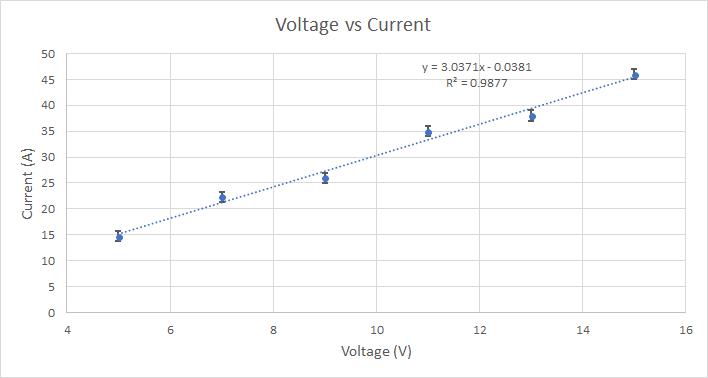
\includegraphics[width=0.9\textwidth]{intro-example-scatter}
\caption{Example of a scatter plot. Each measurement is displayed as a point. One can add error bars in both the x and y axes (although only the y direction is displayed here). One can also fit an equation to the data set.}
\label{Fig:Example-Scatter}
\end{figure}

A scatter plot allows you to see the general trend of your data. If you expect a specific behaviour, you can fit a trendline to your data to match a specific equation. By further plotting error bars, you can compare how far away your data points are from the expected trendline. 
This gives you some insight into whether your data matches your expected trend. From the trendline, you can also see the actual coefficient of the fit. As shown in Fig.~\ref{Fig:Example-Scatter}, you can also display a $R^2$ value, which is called the coefficient of determination. This tells you how good your fit was to your data. A perfect $R^2$ value is $1$. See the appendix \ref{App:R2} for details.
For the example of Fig.~\ref{Fig:Example-Scatter}, the $R^2$ value is good and most of the measurements fall within a standard deviation of the fit, therefore this says that the current is proportional to the voltage by a proportionality factor of $3.0371$. 

In summary, to present your data, you will need to know certain things: how to perform an average and other basic statistics, how to evaluate the uncertainty in your measurements and by extension, the final results you obtain from these, how many digits to display in your final answer, and most importantly, how to analyse your data. This will be the subject of the following sections.

\section{Basic Statistics} \label{Sect:Basic-statistics}

\noindent \large \textbf{Mean (Average)} \normalsize

Let $y(x)$ be a function of $x_i$ data points. The value of $y$ for $x_i$ can be denoted by $y(x_i)$ or $y_i$. The mean, or average, denoted by $\bar{y}$ of a dataset with $N$ datapoints is given by
\begin{equation}
\bar{y} = \frac{1}{N} \displaystyle \sum_{i}^N y(x_i) = \frac{1}{N} \left( y(x_1) + y(x_2) +... + y(x_N) \right).
\end{equation}

\noindent \large \textbf{Standard deviation} \normalsize

The standard deviation of a function $y(x)$ is denoted by $\sigma_y$. One says that a measurement $y(x_i)$ has an \textit{uncertainty} of
\begin{equation}
y_i \pm \sigma_{y_i}.
\end{equation}
The standard deviation tells you up to what value is your data precise: your data point can vary between $y_i + \sigma_{y_i}$ and $y_i - \sigma_{y_i}$. This means that your measurement $y_i$ can vary by $2 \sigma_{y_i}$. A good set of measurement would have a very small standard deviation: this gives you the bounds under which your measurement is considered precise. You will see in section ``\textbf{Error Analysis}" how to calculate this quantity. \\

\noindent \large \textbf{Significant Numbers} \normalsize

To present results, one must present an appropriate number of significant numbers. In this course, we will not be concerned with the \textit{number of significant digits}, but more with consistency in reporting the precision attributed to a measurement. 
When quoting a measurement, the last digit should be fixed by the uncertainty of the measurement: it must match the order of magnitude of the standard deviation. In other words, the standard deviation fixes up to what precision (roughly decimal place) you can quote your results. Table~\ref{Tab:SigFigs} lists some common mistakes and how to present those results appropriately. In the context of this course, we will simplify our conventions by \underline{keeping only one significant number for the standard deviation}. Recall that leading zeros do not count as a significant number and trailing zeros (after the precision of the standard deviation) should be discarded.

\begin{table}[h]
\centering
\begin{tabular}{||c|c||}
\hline
Incorrect & Correct \\ \hline
$324.9453 \pm 0.02$m & $324.95 \pm 0.02$m \\
$20 \pm 0.1$\$ & $20.0 \pm 0.1$\$ \\
 $3 \times 10^4 \pm 2$N & $3000 \pm 2$N \\
$31.02 \pm 0.10$\$ & $31.0 \pm 0.1$\$ \\
$0.003564 \pm 0.00012$m/s & $0.0036 \pm 0.0001$m/s \\ \hline
\end{tabular}
\caption{Significant numbers. Common mistakes and the correct way to present such results.}
\label{Tab:SigFigs}
\end{table}

\noindent \large \textbf{Precision versus Accuracy} \normalsize

\textbf{Precision} refers to how closely related two measurements are from each other. This means that one expects a \underline{small standard deviation} for highly precise measurements.

\textbf{Accuracy} measurements refers to the closeness of a measurement from a \textit{known} value. This means that one must calculate the \underline{difference} of the measurement to the known value \underline{in terms of standard deviations}. For example, if $y=0.4 \pm 0.1$m, and the known value is $y_t=0.7$m, then the measurement differs by $3\sigma_y$.

Often, one may encounter a highly precise set of measurements, but also very inaccurate. This is a signal that there may have been a \textbf{systematic error} in your results. This is a type of error that propagates throughout your experiment and offsets your results by a constant factor. For example, recall the equation of the period of oscillation of a pendulum is
\begin{equation}
T = 2 \pi \sqrt{\frac{L}{g}}.
\end{equation}
If one incorrectly measured the length $L$ of the string, then the results would be offset by a constant factor of $\sqrt{L_{good}- L_{bad}}$. \\

\section{Error Analysis} \label{Sec:ErrorAnalysis}

Measurements carry an inherent uncertainty to them.
To characterize this uncertainty, we write attribute them a value to which the measurement can vary. This standard variation is called a \textit{standard deviation}. For this reason, we will often use is interchangeably with the term \textit{uncertainty}. 
Note that there is a formal mathematical definition of the concept of standard deviation, but for the context of this course, we will abstain of such definition.
Sometimes, a measurement must be manipulated with other measurements in order to obtain another variable. To keep track of how the uncertainty of each measurement is propagate through this manipulation, we use \textit{error propagation} techniques. This characterizes the \textit{error} on this derived quantity, and therefore, it is another type of uncertainty.
Thus, we will also use the term \textit{error} interchangeably with \textit{uncertainty}.\\

\noindent \large \textbf{Standard deviation of a measurement} \normalsize

The \textit{rule of thumb} for finding the standard deviation of measurements is as follows: each measurement can vary by \textit{half} of the smallest available precision from your measuring instrument, and you must add the uncertainties of the measurement. Consider the example of measuring a distance with a 30cm ruler. The smallest increment is a mm. When you measure a distance between \underline{two points}, you take \underline{two} measurements: one at each point. Thus the uncertainty on the measurement is $2 \times 0.5$mm, so $1$mm. This is exactly the smallest available increment of your measuring device. Therefore, unless otherwise specified, the \textit{standard deviation of a measurement is the smallest available measurable value allowed by your instrument}. 

Another example is measuring the time difference between two events. Again, there will be two measurements: the initial and end time. Stopwatches often allow one to view up to ms precision. However, the average visual time reaction is roughly $0.3$s, and therefore each initial and final time measurement varies by $0.15$s and so the uncertainty for the whole measurement is $0.3$s. \\

\noindent \large \textbf{Standard deviation for fluctuating data} \normalsize

For fluctuating datasets where \textit{each measurement is independent of the previous}, to reliably represent your data, you should take some form of average over some number of measurements. Measurements that are random are said to follow a \textit{Poisson distribution}. To study these types of measurements, one typically chooses a subset of $N$ data points, and calculate its mean. Given the mean, one must approximate the error as
\begin{equation}
d_i = y_i - \bar{y}.
\end{equation}
The standard deviation on the average of your measurements will therefore be given as
\begin{equation}
\sigma_{\bar{y}} = \sqrt{ \frac{1}{N} \displaystyle \sum_{i=1}^{N} d_i^2}.
\label{Eq:STDev.P}
\end{equation}
This can be obtained in Excel by using the function \verb|=STDEV.P(x)|. \\

\noindent \large \textbf{Error propagation} \normalsize

The standard deviation value above is attributed to \underline{a single measurement}. However, often one would be interested in deriving a quantity that depends on \textit{multiple} measurements. To describe the standard deviation on the end result, one must use \textit{error propagation techniques}.

For these labs, you will only need to know the following two error propagation formulas. Consider first the following function
\begin{equation}
f(x,y) = x \times y.
\label{Eq:f=xy}
\end{equation}
The standard deviation $\sigma_f$ on $f$ will be
\begin{equation}
\sigma_f = \sqrt{ (x \sigma_y)^2 + (y \sigma_x)^2}.
\label{Eq:product error}
\end{equation}
This will be useful for example to calculate the error on the area given two length measurements, or in Lab 2, you can calculate the error on the time constant in a similar way.

Consider also the function
\begin{equation}
f(x) = \frac{1}{x}.
\label{Eq:f=1/x}
\end{equation}
The standard deviation for this case is
\begin{equation}
\sigma_f = \frac{\sigma_x}{x^2}.
\label{Eq:1/x error}
\end{equation}


\noindent \large \textbf{Measurement analysis} \normalsize

To understand the significance of a measurement, one can compare it in different ways. When a theoretical value is known, one can compare a set of measurements by calculating the \textit{absolute error}, the \textit{percentage error} or the \textit{standard deviation error}. One can also analyse a dataset by studying fits in a similar manner. \\

\noindent \textbf{Absolute error}

The absolute error indicates the difference between the known value, and either a measurement, the mean value of a set of measurements, or a fit parameter. One can also compare a set of measurement to the fit of the dataset in this matter. Let $y_t$ be the theoretical value and $y$ be one of the variables mentioned before, then the absolute value is
\begin{equation}
\text{Absolute error} = \left\rvert y_t - y \right\rvert
\end{equation}

\noindent \textbf{Percentage error}

The percentage error is simply the ratio of absolute error relative to the known value. This gives an indication, in percentage, of how far away with respect to the known value is the measurement. It is given as
\begin{equation}
\text{Percentage error} = \left\rvert \frac{y_t - y}{y_t} \right\rvert \times 100
\end{equation}

\noindent \textbf{Standard deviation error}

The standard deviation error indicates how many standard deviations away is a measurement when compared to the known value. It is given as
\begin{equation}
\text{Standard deviation error} = \left\rvert \frac{y_t - y}{\sigma_y} \right\rvert
\end{equation}

You will have to recognize which one of the above is useful and representative of the information that you wish to convey for the data analysis that you have to perform. Note that we've taken the absolute values of the above, but by not doing so, we could convey information about the ``direction" of the error i.e. whether the measurements are higher or lower than the known theoretical value.\\

\noindent \large \textbf{Fit analysis} \normalsize

As mentioned before, a good way to know whether your fit is correct is to compute the coefficient of determination $R^2$. To compare your fit to your data, you should see whether your data points all (or mostly) fall within one standard deviation of the fitted equation, that is if the standard deviation error should be less than 1 $\sigma$ for all data points when compared to $y_{fit}$.
Note that for small $R^2$, it could be possible that the fit falls within the error bars of your graph, and therefore
one would like to obtain $R^2\approx 1$ with small error bars.

It is worth mentioning that in realistic settings, what is considered a ``good" $R^2$ value varies depending on context.
In physics, simple models can yield $R^2\approx 1$. 
In contrast, a good $R^2$ value in biological systems can be in the range of $0.7$,
and in social sciences, the standards are often lower.
This highlights the quantitative nature of physics and its eloquent relation to mathematics, and therefore
this serves as an optimal stage for you to learn about quantitative data analysis.	


\part{Lab Manuals} \label{Part:Labs}

\chapter{Lab 1 - Capacitance}
\section{Learning objectives}
\begin{itemize}
\item How to acquire data
\item How to quantify error
\item How to present data
\item Learn about linear fits
\item Confirm capacitance law
\end{itemize}


\section{Introduction}
In this lab you will be asked to accomplish the following tasks:
\begin{itemize}
\item Find possible parameters that could affect the capacitance of a parallel plate capacitor system.
\item Support your conclusion based on a quantitative evaluation of your data.
\end{itemize}

You will have to chose some parameters and quantify their affect on the capacitance of the setup. In the process, you will learn how to acquire good data and how to quantify and present your data. We would like to re-emphasize that collaborations and discussions are encouraged and expected throughout the two sessions of the lab.

In the first session, you will work together to find possible parameters that can affect the capacitance of a pair of parallel plates. Measurements at this stage may be crude; do not worry about that, we are {\it not} evaluating the usefulness of the data at this stage, rather the process of thinking about what this data {\it means}, and your thinking process about how to improve your experiment to obtain better data.

During the second session, you will be asked to obtain quantitatively improved data and to compare it with data from the previous session. You must then conclude, based on a quantitative evaluation of your data, whether or not, and how, your chosen parameter affects the capacitance of a parallel plate capacitor. \\

\subsection{Pre-lab activity}
To answer some of these questions, we encourage you to review Chapter \ref{Ch:Data-analysis} of the lab manual on  \textbf{Data Analysis}.
\begin{enumerate}
\item What is a measurement? Give your own definition of what constitutes a measurement based on your previous courses with lab components (biology, chemistry, physics).
\item Two engineers must measure the distance between the McGill metro station to the athletic centre to build an underground tunnel. One engineer finds that the distance is $9134 \pm 5$m while the other finds that the distance is $9150 \pm 20$m. In what ways can they compare their measurements? Do their measurements agree? Explain.
\item The city is considering to build a metro line between McGill station and the station at University of Montreal. To do this, an engineer decides to use a km-long ruler whose smallest divider is a meter. She \textit{did not} use any other measuring devices. She takes her measurements and presents her findings to her team as $3653.4500$m. What is the uncertainty on this measurement? Did she present enough, too little or too many digits about her measurement? Why?
\item Two groups of researchers are trying to test their new methodology to measure the speed of light $c$. Current research shows that the speed of light is roughly $c=2.99 792 \times 10^8$ m/s. The first group finds that $c=2.88 \pm 0.02 \times 10^8$ m/s while the second group finds that $c=3.0 \pm 0.2 \times 10^8$ m/s. What do these measurements tell you about their methodology in the context of precision and accuracy? What type of mistake may have caused the discrepancy in the first group's results?
\item How do you know if an experimental result is acceptable and trustworthy? What gives you confidence that your data is trustworthy?
\end{enumerate}

\subsection{What is a capacitor?}
You  learned in class that charges can attract and repel each other. This is because point charges source \textit{electric fields} that apply a force on a test charge. Since there exists a force between two point charges, there exists a \textit{potential energy difference}  $\Delta U$ between two point charges (relative to some reference separation) due to this force. We define  \textit{electrical potential difference} as \textit{the potential energy difference  \underline{per unit charge}}, 
\begin{equation}
\Delta V = \frac{\Delta U}{q}
\label{Eq:ElectricPotential}
\end{equation}
where here $q$ is the \textit{charge of a test particle} displaced in the electric field of a source charge $Q$. In practice, it is more useful to define an electrical potential difference to move \textit{\underline{any} test charge} $q$ from $r=\infty$ to a distance $R$ from a source charge $Q$ as
\begin{equation}
V = \frac{k Q}{R}
\label{Eq:ElectricPotential_point}
\end{equation}
where $k$ is Coulomb's constant $k = {1}/{4\pi \epsilon_0}$. This will have units of \textit{voltage} V. This process is depicted in Fig. \ref{Fig:ElectricPotential_point}.
\begin{figure}[h]
\centering
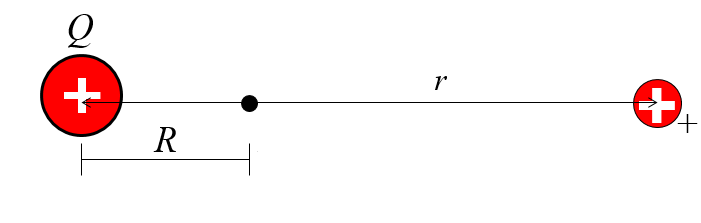
\includegraphics[width=0.7 \textwidth]{lab1-electric-potential.png}
\caption{The electrical potential due to a source charge $Q$ (left) at a distance $R$. The test charge (right) is placed at a distance $r$ from the location that we measure the electrical potential difference.}
\label{Fig:ElectricPotential_point}
\end{figure}

Now consider a pair of parallel conducting plates separated by a distance $d$ connected to a battery as shown in Fig.~\ref{Fig:ParallelPlates}. A pair of parallel plates separated by air or another (non-conducting) material can be assembled into a \textit{capacitor}: on each parallel plate, because of the battery, there will accumulate a number of equal and opposite charges: electrons on the negative plate such that the total charge is $-Q$, and $+Q$ will accumulate on the positive plate. Because of the gap (separation) between the plates, there now exists an electric potential between the plates, which is given by eq.~\eqref{Eq:ElectricPotential}.
\begin{figure}[h]
\centering
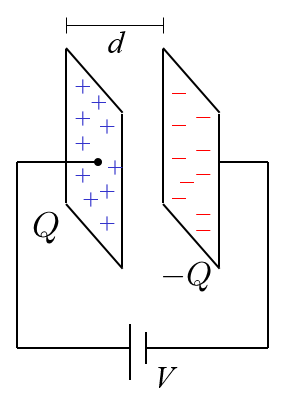
\includegraphics[scale=0.6]{lab1-parallel-plates.png}
\caption{Parallel plate setup. The battery with voltage $V$ creates a flow of electrons such that there will accumulate a total charge of $-Q$ on the negative plate, and $+Q$ on the positive plate. Since the plates are separated by a distance $d$, there will be a electrical potential difference between the two plates.}
\label{Fig:ParallelPlates}
\end{figure}

One defines the \textit{capacitance} of a capacitor as the constant of proportionality between the total number of charges $Q$ (same magnitude on either plate) and the electric potential $V$ stored between the plates, i.e. 
\begin{equation}
Q = C V.
\label{Eq:lab1-Q=CV}
\end{equation}
Capacitance is measured in Farads F.  In this lab, you will be asked to verify \textit{what} affects the capacitance $C$ of a parallel plate capacitor system. (A useful constant in such setup is the \textit{vacuum permittivity} $\epsilon = 8.85 \times 10^{-12}$F/m.)


\section{Protocol}
\subsection{Session a}
The available materials to be used in your experiments are listed in Table \ref{Tab:Lab1-material}. The metallic rectangular plates will be of varying dimensions. The manipulations are straightforward: insert either a plastic or paper sheet between the two plates and use the Arduino unit (see below) to measure the capacitance. At this point, you do not need to know how the Arduino unit works, simply how to use it. You will learn how it works in the next lab. The plates must not touch each, otherwise you will not see a measurement: this causes a short-circuit and therefore you will not see a capacitance measurement. You can assume that the distance between the plates is the thickness of the plastic or paper sheet.
\begin{table}[h]
\centering
\begin{tabular}{||c | c ||}
\hline
Individual station & Collective station\\ \hline
Laptop & Aluminum foil \\
Arduino capacitance setup & Blocks of wood \\
Metallic plates & Small weights \\
30cm ruler & Assorted capacitors \\
Plastic sheets & Assorted resistors \\
Paper sheets & Extra wires \\
& Micrometer \\
& Multimeter \\
\hline
\end{tabular}
\caption{Available material for Lab \# 1}
\label{Tab:Lab1-material}
\end{table}

\noindent Information about using the Arduino code can be found \href{https://www.arduino.cc/en/Tutorial/CapacitanceMeter}{here}. To use the Arduino unit:
\begin{enumerate}
\item Plug the USB-port into the laptop
\item Open the Arduino Genuino application on the laptop.
\item Open the capacitanceMeter.ino file found by opening Windows Explorer and typing \url{\\\\altima\\Physics_DFS\\Physics_102} in the address bar.

\item In the tabs above, go into the drop-down menu Tools $\rightarrow$ Port. Choose whichever COM is labelled by ``(Arduino/Genuino Uno)".
\begin{figure}[H]
\centering
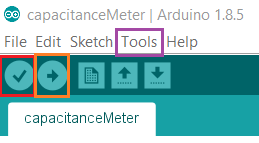
\includegraphics[width=0.5 \textwidth]{lab1-Arduino-menu-bar.png}
\caption{Arduino application menu bar. Note that the color boxes were added to guide the eye. The red checkmark box is the \textbf{verify} button. It serves to verify whether there is an error in the code. The orange right arrow box is the \textbf{upload} button, and the purple box is the \textbf{Tools} drop-down menu bar.}
\label{Fig:ArduinoMenuBar}
\end{figure}

\item Verify the script by clicking the icon with the checkmark. If there is an error, call the TA.
\item Upload the script by clicking the icon with the right arrow.
\item In the tabs above, go into Tools $\rightarrow$ Serial Monitor (or on your keyboard, press Ctrl+Shift+M). You should see that a window open as follows (without the numbers):
\begin{figure}[h]
\centering
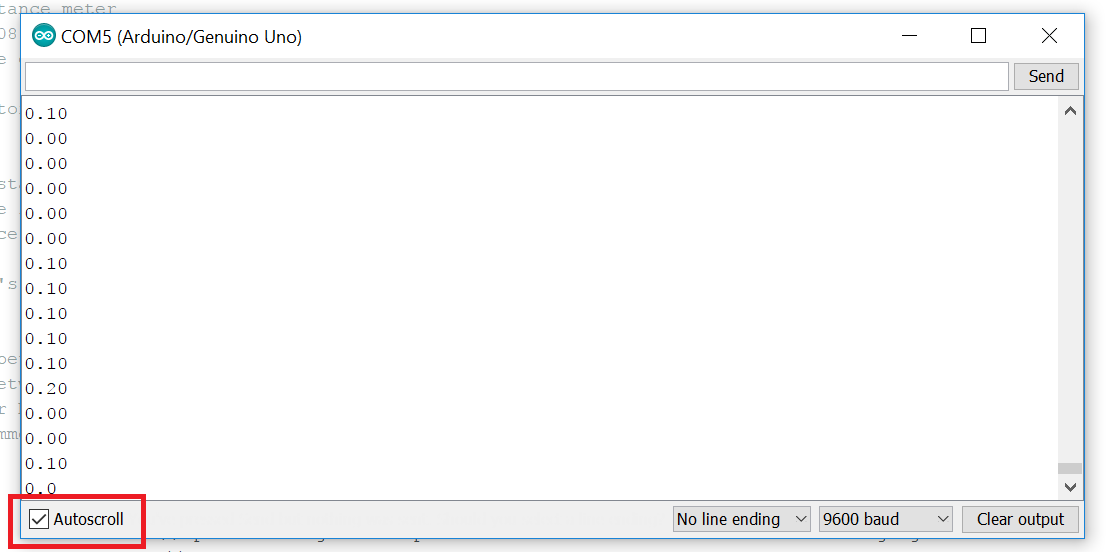
\includegraphics[width=0.85 \textwidth]{lab1-Arduino-monitor.png}
\caption{Arduino Serial Monitor. This is a pop-up screen where you will see your capacitance measurements scroll by. The Arduino unit takes a capcitance measurement at a fixed frequency. Unless otherwise specified, the output is in nanoFarads. Units aren't displayed so as to simplify the transfer from the monitor screen to Excel, but one could display the units by changing the command in the Arduino script. To stop the scrolling of measurements, click on the Autoscroll box.}
\label{Fig:Arduino-Monitor}
\end{figure}

\item Take the two wires (see Fig.~\anhkhoi{updated setup}) and simply touch each side of the parallel plates: you should see a multitude of measurements scrolling down the monitor window, as in Fig.~\ref{Fig:Arduino-Monitor}. If you do not see many measurements scrolling in the monitor window, it is likely that the plates are touching each other and you therefore have a short circuit. \anhkhoi{input new setup pic}
\item You can stop the auto-scroll by clicking the bottom-left box to better see your results (see Fig.~\ref{Fig:Arduino-Monitor}).
\end{enumerate}

Notice that in Fig.~\ref{Fig:Arduino-Monitor}, the data fluctuates. You will have to determine how many capacitance measurements  you should average over to acquire a good representation of a particular capacitance measurement. 
We refer you to the Part I, section \ref{Sec:ErrorAnalysis} of the lab manual. Using this setup, proceed to conduct you experiments and collect data that will let you evaluate $C$ in eq.~\eqref{Eq:lab1-Q=CV} as a function of different geometrical parameters of the capacitor system. 

You will have the opportunity to test whatever hypothesis you may have, however \textbf{every group must at least include a capacitance measurements for \underline{three} or more different pairs of plate sizes while inserting a single sheet of plastic between them. 
The plates must be perfectly aligned on top of each other}. After doing so, you may explore in more details the consequences of these measurements, or you may study other possible parameters that could affect the capacitance.

Given the measurement of the two sides $L_1$ and $L_2$ of a rectangle and their corresponding standard deviations $\sigma_{L_1}$ and $\sigma_{L_2}$, the standard deviation on the area is given by
\begin{equation}
\sigma_A = \sqrt{ \left( L_1 \sigma_{L_2} \right)^2 + \left( L_2 \sigma_{L_1} \right)^2 }.
\end{equation}

While studying other parameters, if you are unsure of the standard deviation of a certain parameter, you may ask the TAs to help derive the appropriate derived standard deviation for that parameter.

To analyse your data, we refer you to section \ref{Sec:lab1-analysis}.
{\color{blue}Enter your set up, measurement process and data in your log book.} Before handing in your log book, be sure to write down your {\color{blue}observations in the \textbf{General Notes} section of your log book, and a rough plan of what you intend to do during the next session in the \textbf{Conclusions and future work} section}. The latter part should be done after discussions with at least one other group.

\subsection{Session b}

We recommend that you bring whatever material that you think could help you acquire better data in Session b. 
By now, you should know what parameters affect the capacitance, and therefore you should plan in advance your own ``protocol" to verify your hypothesis quantitatively with improved data, compared to that in Session a. 
This protocol does \underline{not} have to match what you wrote in your log book in Session a, but if it does differ, you must explain what made you change your mind.

{\color{blue} We expect that you contrast your results from this session versus those you obtained in the previous one: explain how your measurements improved or differed.}

{\color{blue}Be mindful that you will be evaluated based on your data presentation, data analysis and explanation of the physics from this session, therefore be certain to \textit{fully, but succinctly, describe} your thought process.} 

\section{Measurement Analysis}
\label{Sec:lab1-analysis}
During this lab, you will have to use data analysis techniques to understand your data. For \underline{each session}, we recommend that you analyse your data as follows.

To study a system, one typically isolates as many variables as possible to see each of its individual affect on the whole system. If we are able to isolate such a variable, mathematically, that is the equivalent of finding some $f(x)$ that depends just on one variable $x$. In this lab, you will find as many variables that can affect the capacitance as possible by isolating each such variable, one at a time.

For each dataset, corresponding to each parameter you measure, you must abide by the error analysis rules outlined in chapter \ref{Ch:Data-analysis}. 
The data analysis can be done much more rapidly with Execl spreadsheets, therefore we highly recommend that you read appendix \ref{App:Excel}. 

Once you have  result from your data, you must offer a physical explanation that supports your results. {\color{blue} Explain why physically each parameter affects the capacitance of the system. Support any claims you make by proposing a possible experiment to test your claims, and offer possible outcomes that one could observe from your experiment.} Recall that bouncing your ideas off peers is an invaluable way to actually test the rational of your hypothesis.

\chapter{Lab 2 - RC Circuits}
\section{Learning objectives}
\begin{itemize}
\item Learn how to connect circuits
\item Learn about exponential functions
\item Learn about RC circuits
\item Learn about equivalent resistance and capacitance
\end{itemize}

\section{Introduction}
In this lab you will characterize an RC circuit. An RC circuit is a circuit that contains a resistor (R) and a capacitor (C), connected in series with an EMF source during charging and without the battery during discharging.  
The data analysis tool we will use is called a PASCO 850 Universal Interface, the use of which will be explained below. 
Specifically, we will  use a voltmeter and a 
signal generator tool to examine the charging and discharging of a capacitor. 

In the first lab session, you will be asked to \textbf{measure the time constant} $\tau$ of a given RC circuit (more on tbis below). 
In the process, you will learn how to measure time constants and understand subtleties in the data acquisition apparatus. 
This session will be more like a traditional lab where you will follow well outlined instructions. 

In the second session, you will be asked to \textbf{build an RC circuit with a specific time constant} and to show, based on well supported data, that your circuit has the appropriate time constant. 
When you arrive at the second session, you will receive a sheet that asks you to build an RC circuit with a specific number of parallel branches. 
You will have to deduce how to choose an appropriate number of resistors and capacitors for these branches to obtain a specific time constant.

\subsection{Pre-lab activity}
\begin{enumerate}
\item Why would we want to fit a dataset to an equation?
\item What is $e^{x}$ evaluated at $x=0$, $x=1$ and $x=-1$?
\item For $f(x) = e^{-x}$, what is the value of $x$ so that $f(x)=0$?
\item What does $a$, $b$ and $c$ do in the following function?
\begin{equation}
f(x) = a e^{b x}+c
\end{equation}
\item What is the difference between these two plots:
\begin{figure}[h]
\centering
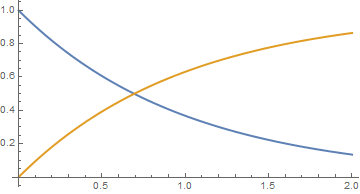
\includegraphics[width=0.8\linewidth]{lab2-prelab}
\caption{Exponential functions.}
\label{Fig:lab2-prelab}
\end{figure}
\end{enumerate}

\subsection{RC Circuits}
Recall that the capacitance is defined as the proportionality constant between the total charge accumulated by a capacitor and the voltage difference across the circuit
\begin{equation}
Q = C \Delta V.
\end{equation}
In this equation, the charge $Q$ is expressed in Coulomb (C), the voltage $\Delta V$, in volts (V) and the capacitance $C$ in farads (F).

In this lab you will study both the \textit{charging} and \textit{discharging} process of an RC circuit. 
During the charging process, an electrical EMF source accumulates charges  on each side of the parallel plate capacitor.
During the discharging process, the capacitor releases all its charges into the circuit (which now does not contain the battery). 
Capacitors charge and discharge exponentially in time. 
During the \textit{discharge} of a capacitor, the instantaneous voltage $\Delta V_C$ between the ends of the capacitor also drops and is given by
\begin{equation}
\Delta V_C = \Delta V_{max} e^{-t/\tau}
\label{Eq:V-discharge}
\end{equation}
where $\Delta V_{max}$ is the maximum voltage across the capacitor, i.e. the voltage to which the capacitor was initially charged, $t$ is the time and $\tau$ is the \textit{time constant} given by
\begin{equation}
\tau = R_{eq} C_{eq}
\label{Eq:time-constant}
\end{equation}
where $R_{eq}$ and $C_{eq}$ are, respectively, the equivalent resistance and capacitance to which we can reduce the circuit. 
Although the theoretical discharge time is infinite, in practice we consider that the discharge is over when the voltage at the bounds of the capacitor is at $1\%$ of its maximal value. 

\subsection{Equivalent resistance and capacitance}
To find the equivalent resistance and capacitance of a circuit, one must apply the correct equations to sum the contributions of all the components. 
The equivalent quantity differs depending on whether the resistors and capacitors are combined in series or in parallel. For resistors, the equivalent resistance is given as
\begin{equation}
R_{series} = R_1 + R_2 + R_3 + ... R_n = \displaystyle \sum_{i=1}^n R_i
\end{equation}
\begin{equation}
\frac{1}{R_{parallel}} = \frac{1}{R_1} + \frac{1}{R_2} + \frac{1}{R_3} + ... + \frac{1}{R_n} = \displaystyle \sum_{i=1}^n \frac{1}{R_i}
\end{equation}

For capacitors, the equivalent capacitance is given as
\begin{equation}
C_{parallel} = C_1 + C_2 + C_3 + ... C_n = \displaystyle \sum_{i=1}^n C_i
\end{equation}
\begin{equation}
\frac{1}{C_{series}} =  \frac{1}{C_1} + \frac{1}{C_2} + \frac{1}{C_3} + ... + \frac{1}{C_n} = \displaystyle  \sum_{i=1}^n \frac{1}{C_i}
\end{equation}

\subsection{Data Acquisition  Equipment} \label{Sect:lab2-equipment}
In this lab you will use the PASCO 850 Universal Interface to measure and plot voltages as a function of time in an RC circuit. 
We will use two terminals of the PASCO device. The first connects to the input/output voltage source. 
The other (Analog connectors) is a pair of probes which measures the voltage across the capacitor of the circuit. 
See Fig.~\ref{Fig:lab2-PASCO} for location of terminals.

\begin{figure}[h]
\centering
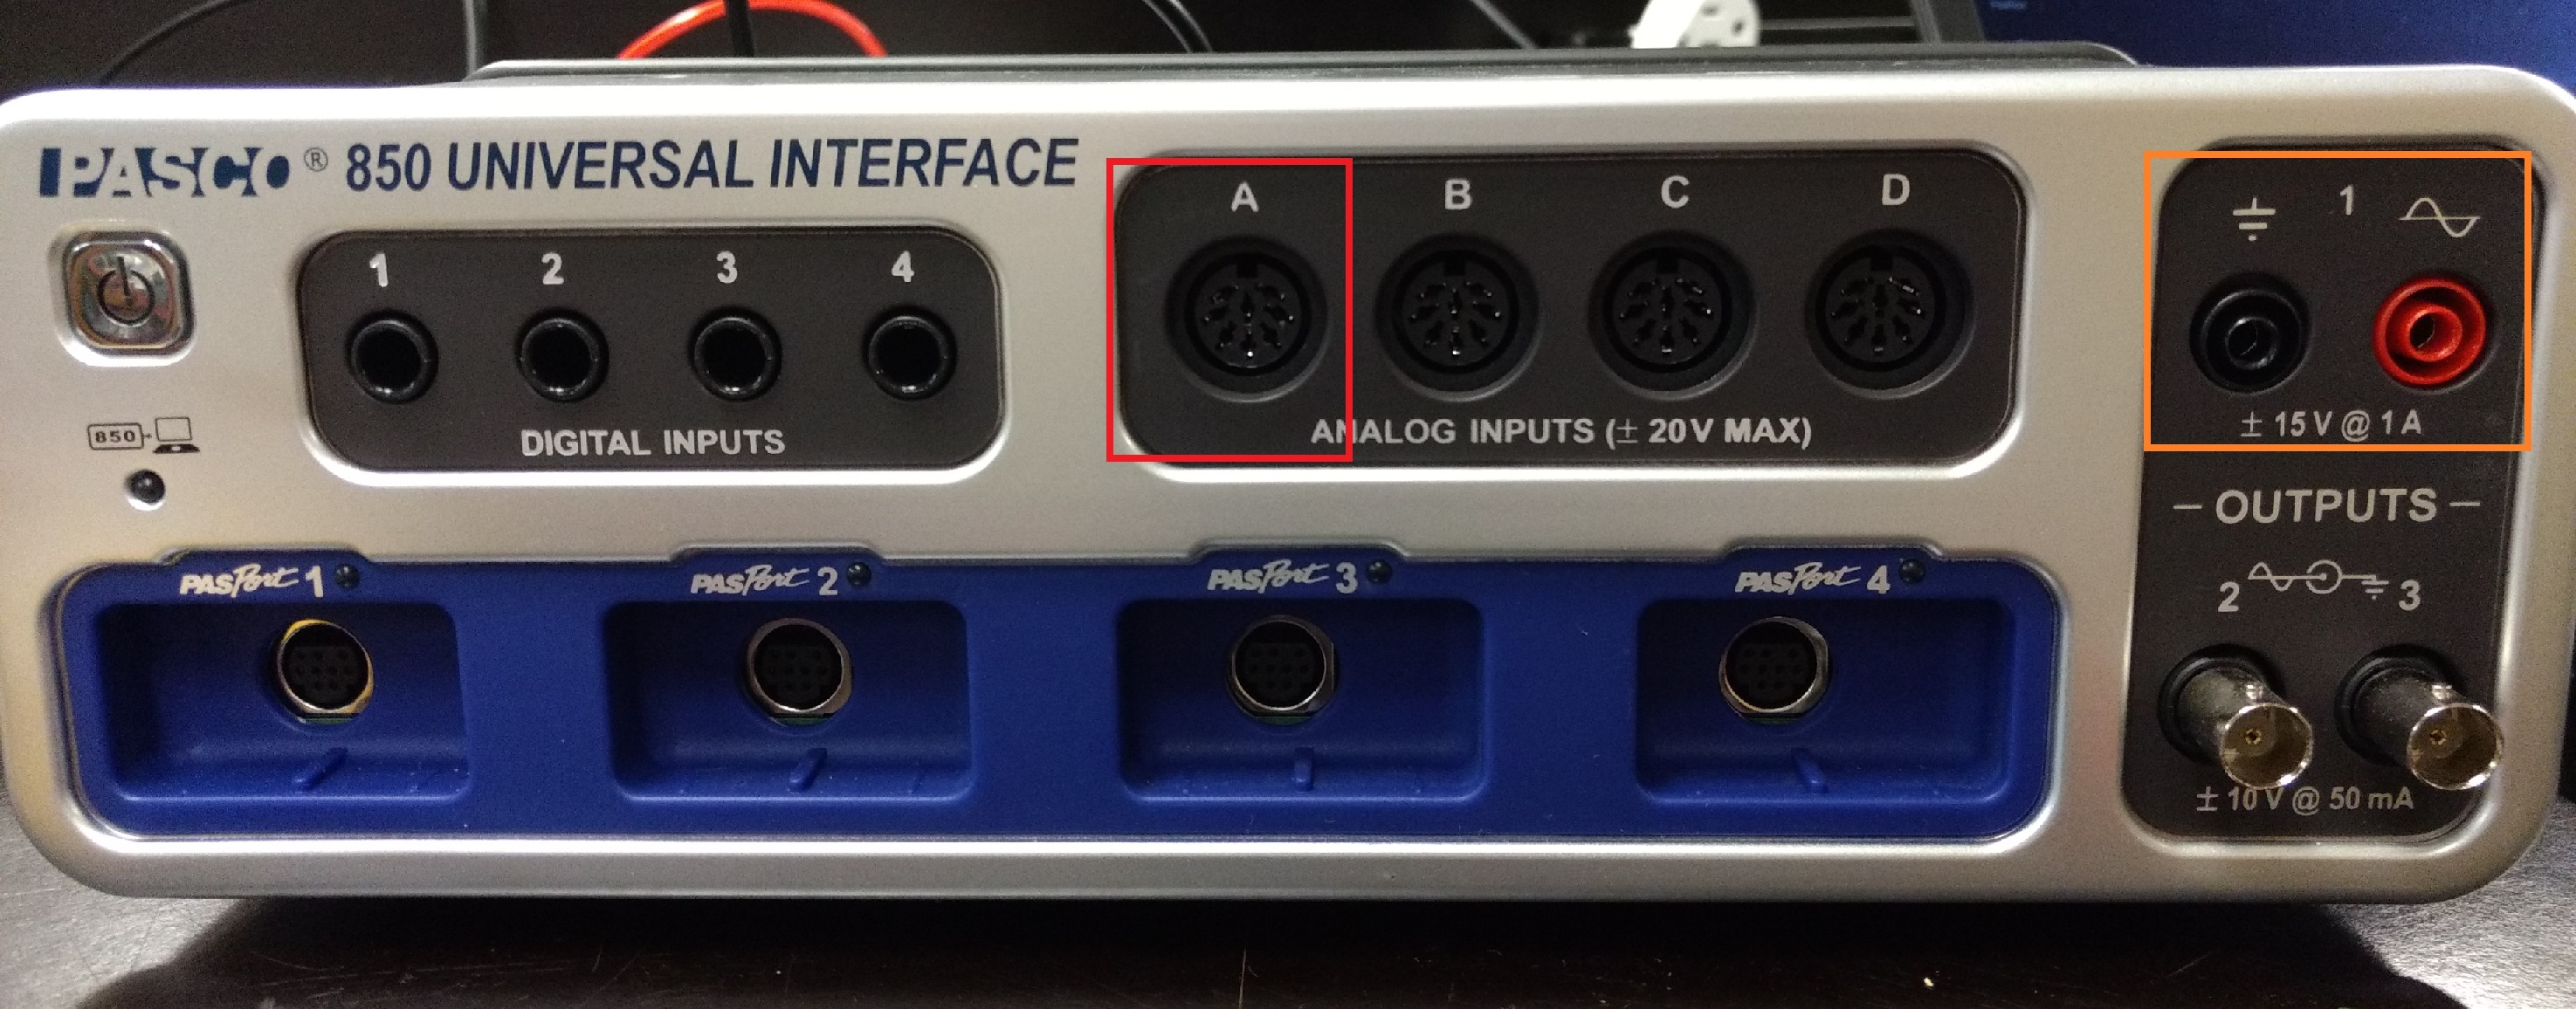
\includegraphics[width=0.8\linewidth]{lab2-PASCO}
\caption{PASCO 850 Universal Interface The red box is the probe Analog input. The voltage source (Output 1) is boxed in orange.}
\label{Fig:lab2-PASCO}
\end{figure}

Given the nature on these measurements, there is an inherent fluctuation to the data that is difficult to characterize. 
During the first session, you are not required to produce quantitatively well supported data: unless otherwise specified, you will not need to keep track of standard deviations.
For the second session, you can completely ignore standard deviations. You are still required to generate $R^2$ values or other quantities that might be relevant to your goal. 


\section{Session a}
\noindent \large \textbf{Hooking up the Equipment} \normalsize \\
During the first session, you will receive an RC circuit fastened onto a wooded board. 
Before proceeding with measurements related to charging and discharging capacitors, conduct the following steps:
\begin{enumerate}
\item Turn the wooden board over to reveal the circuit Fig.~\ref{Fig:lab2-session1-circuit1}. 
There are actually two circuits here, one consisting of a $100$k$\Omega$ rheostat (variable resistor) and the $100\mu$F capacitor, the other consisting of a $470\Omega$ resistor and a $0.1\mu$F capacitor. 
We will not use the $0.1 \mu$F capacitor, or the rheostat.
\item Connect the Output 1 of the PASCO 850 Universal Interface to the wooden board's terminals as well as the Analog Input A in order to complete the circuit as shown on Fig.~\ref{Fig:lab2-session1-circuit1}. 
The $100\mu$F capacitor can now charge through the $470\Omega$ resistor (when in the ``charge" state on the wooden board) and discharge through the $150$k$\Omega$ resistor (when in the ``discharge" state). 
The charging voltage is read on the computer as Input A measures the voltage across the 100$\mu$F capacitor. 
The Output 1 is the one with the red and black connectors and the analog inputs are labelled with letters on upper half of the interface and on the right.
\end{enumerate}

\begin{figure}[h]
\centering
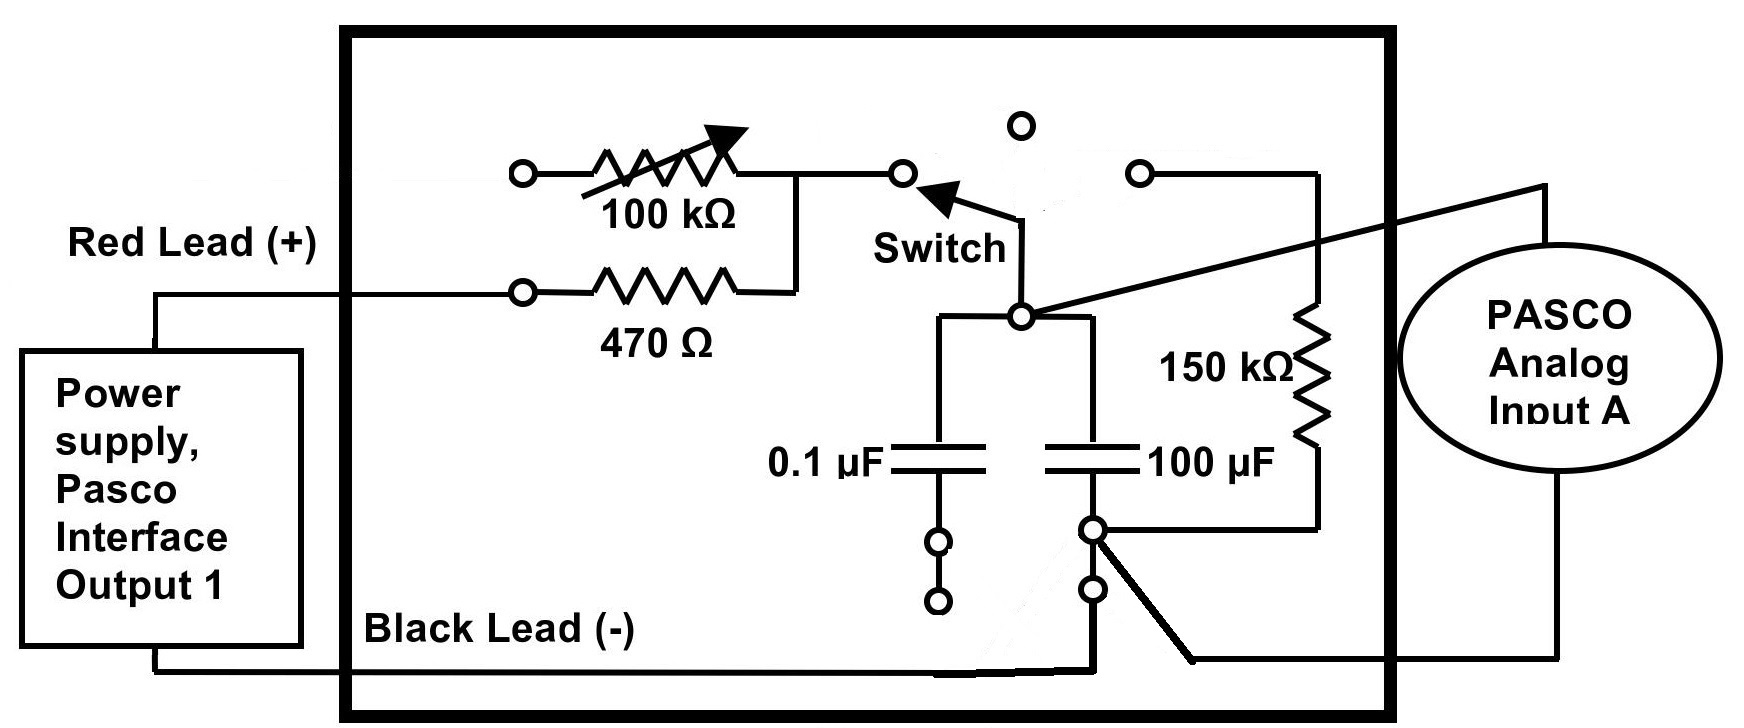
\includegraphics[width=0.75\linewidth]{lab2-session1-circuit2}
\caption{Circuit for session 1.}
\label{Fig:lab2-session1-circuit1}
\end{figure}


\noindent \large \textbf{Protocol} \normalsize \\
You will execute the following steps in order to understand how to use the PASCO interface to characterize an RC circuit. 
For this session, we recommend that you {\color{blue} record your measurements in an Excel spreadsheet, and rewrite the relevant results in your log book and your observations in the General Notes section of your log book. You must also answer the questions that are embedded in the following instructions in the Results part of your log book. You should also write down any technical notes about the apparatus and how an RC circuit works in order for you to fast-track your manipulations for the next session.}

\begin{enumerate}
\item Connect the circuit as shown in Fig.~\ref{Fig:lab2-session1-circuit1} and explained above.
\item The PASCO file can be found by opening Windows Explorer and typing \url{\\\\altima\\Physics_DFS\\Physics_102} in the address bar.
\item Turn on the PASCO and plug in the USB into the computer.
%\item On the software, open the ``Signal Generator" tool, which is located on the left hand side panel and make sure that the signal is set to be DC (Waveform option), has an amplitude of $6V$ and has a data acquisition frequency of $10$ Hz. See Fig.~\ref{Fig:lab2-interface-dc}.
%\begin{figure}[h]
%\centering
%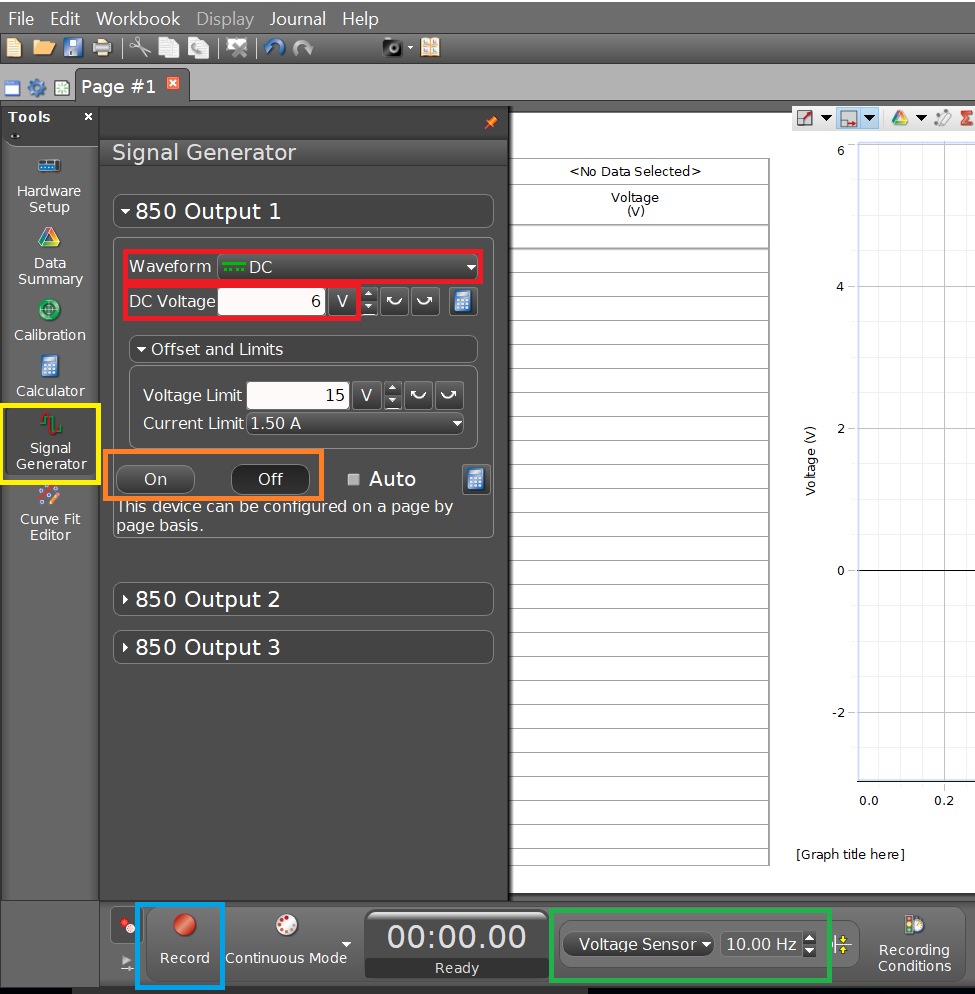
\includegraphics[scale=0.5]{lab2-interface-dc}
%\caption{Settings for a DC waveform input. To find this toolbar, select the ``Signal Generator" tool (yellow box). The red boxes are to set the waveform of the input and the amplitude. Set the data acquisition frequency to 10Hz (see green box). To turn On or Off the signal generator, see the orange box. To record data, select the red recording button (boxed in blue). }
%\label{Fig:lab2-interface-dc}
%\end{figure}

%\item Set the rheostat to its maximum value (turn fully clockwise).
%\item Press the red round Record button, on the bottom panel .
%\item On the computer, under the 850 Output 1, press On to turn on the power supply.
%\item Flip the switch to the ``Charge" position. A graph should slowly appear on your screen. Log the time it takes for the capacitor to charge.
%\item When the capacitor is charged, press the red button that now says Stop.
%\item Press that same button that now says Record and set the switch to discharge the capacitor and notice the rate of the voltage drop. When the capacitor is discharged, stop the recording.
%\item Repeat steps 5 to 8 for the rheostat at approximately half its value and at its minimum value. Compare the charging rates from step 8 (with the maximum rheostat value) with these two new rheostat values. Discuss your qualitative observations in the ``General notes" section of your log book.
%\item Discharge the capacitor (steps 9,10) and record it for the minimum rheostat value. 
%The software can perform an exponential regression on the data you record. To make good use of that, activate the Curve Fitting option (see Fig.~\ref{Fig:lab2-interface-graph}). The curve of eq.~\eqref{Eq:V-discharge} will be fit to the whole data set. To fit it on the right segment on the data set, use the highlighting tool and select/box the values that are most relevant. The time constant is given by the parameter $1/B$ in the curve fitting data window. The error is given by eq.~\eqref{Eq:lab2-error-tau-fit}.
%\begin{figure}[h]
%\centering
%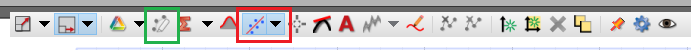
\includegraphics[width=0.9 \linewidth]{lab2-interface-graph-tools}
%\caption{Graphing toolbar. The toolbar appears when moving the mouse to the top of the graph. The red boxed icon is the Curve fitting tool. Select the ``Natural Exponential" function. The highlighting tool is boxed in green. This allows to select a smaller subset of data to apply the curve fitting.}
%\label{Fig:lab2-interface-graph}
%\end{figure}

%\item \textbf{Determine the time constant $\tau$ of the circuit}. $\tau = RC$ is the time the voltage takes to decrease from its maximum value $V_0$ to $1/e$ of $V_0$ (see Section 19.6 of your notes). Use the discharge data from the PASCO in step 12 to determine this. How does the value obtained from the data compare to the fitting exponent provided by the software regression in step 12?
%\item The capacitance value of $100 \mu$F is only approximate. \textbf{Determine} the true capacitance from the time constant measured in step 13 and recalling that $\tau=RC$ (assume that the resistance of $150$k$\Omega$ is correct).
%\item When a capacitor is discharging, the formula is $Q=Q_{max} e^{-t/\tau}$ while when it is charging, the equation is $Q=Q_{max} (1 - e^{-t/\tau})$. What is the difference between the $(1-e^{-x})$ and $e^{-x}$ functions? Explain this in your log book.


%\item We will now learn how to obtain time constants from square wave inputs: we must first connect the 470$\Omega$ resistor in series with the $100\mu$F capacitor as shown below.
%\begin{figure}[h]
%\centering
%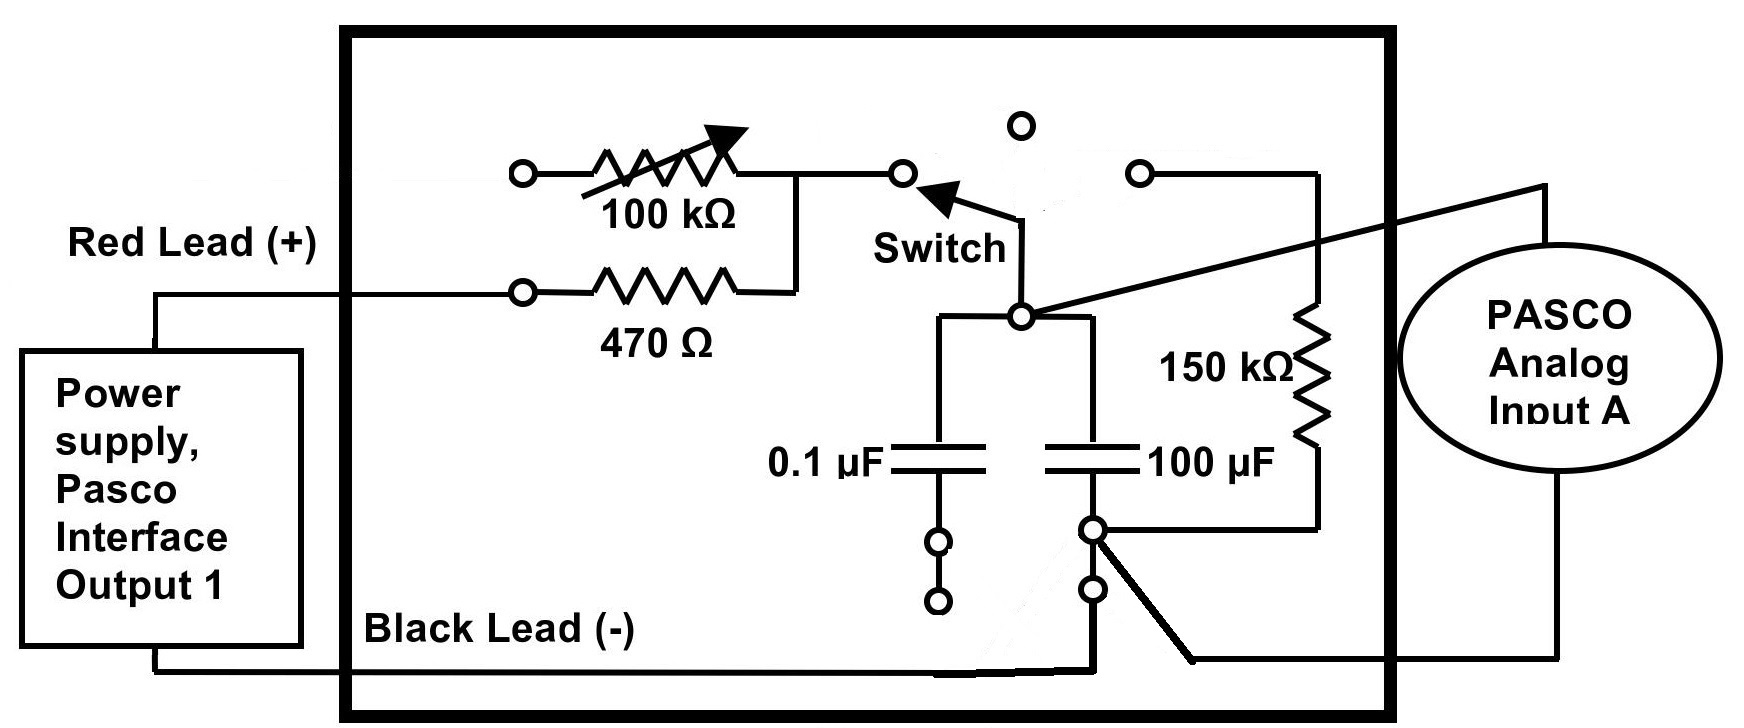
\includegraphics[width=0.75\linewidth]{lab2-session1-circuit2}
%\caption{Connection of the circuit for the $470\Omega$ resistor in series with the $100\mu$F capacitor. By leaving the switch at the position shown, both charging and discharging constants should be the same.}
%\label{Fig:lab2-session1-circuit2}
%\end{figure}

\item In the software, open the ``Signal Generator" tool, which is located on the left hand side panel and make sure that the signal is set to "Positive Square Wave" with an amplitude of 6V and frequency of 0.5 Hz. 
This is equivalent turning on and off a DC voltage 2 times per second. Change the data acquisition frequency found at the bottom of the interface to $1$kHz. See Fig.~\ref{Fig:lab2-interface-square-wave}.
\begin{figure}[h]
\centering
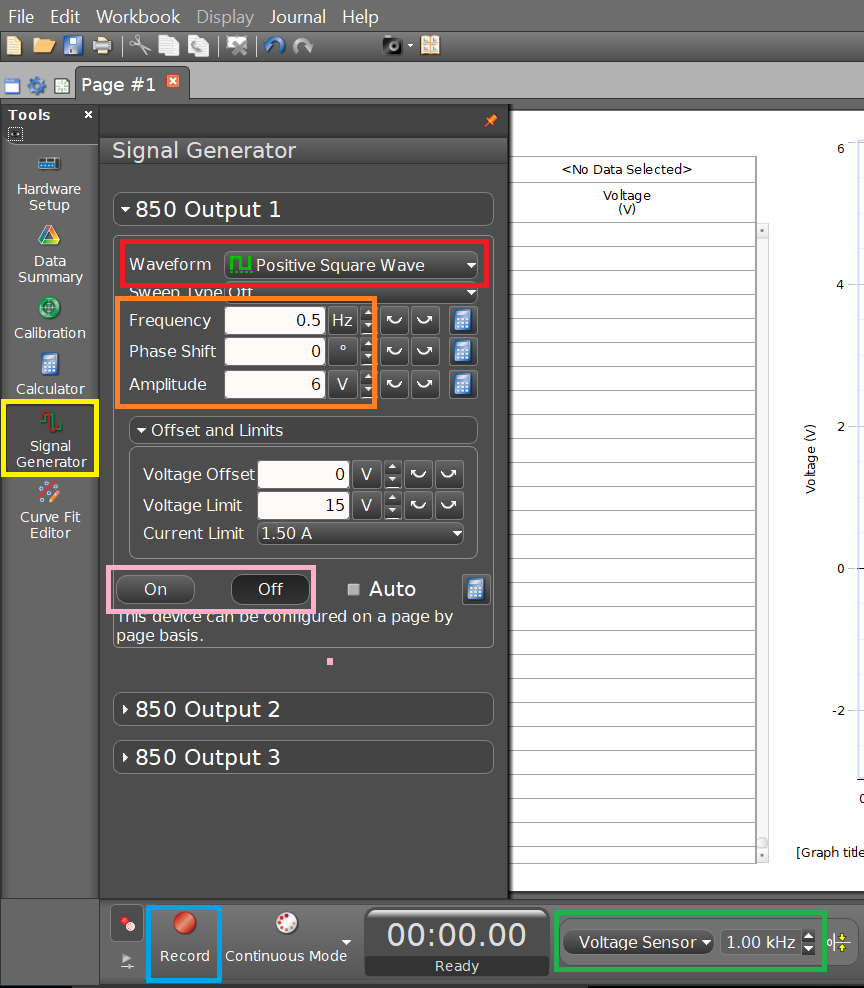
\includegraphics[scale=0.5]{lab2-interface-square-wave}
\caption{Settings for a positive square wave input. You must first select the ``Signal Generator" setting in the yellow box. 
The red box allows to change the waveform. Change the frequency and amplitude according to the orange box. 
Change the data acquisition frequency to the values in the green box. Once you are ready to record your data, select the record button (blue box), and turn on the voltage source (pink box)}
\label{Fig:lab2-interface-square-wave}
\end{figure}

\item With this input from the "Signal Generator" you won't need to use the "charge" and "discharge" switch from the wooded board. Instead you will simply turn On and Off (pink box) the power supply under the 850 Output 1 panel above the 850 Output 2 panel before and after recording measurements. So leave the switch on ``charge" for the rest of the experiment.
%\item Since your time constant is smaller than what you observed from discharging through the $150$k$\Omega$ resistor, you will not need to record data for long.

\item After turning on the signal generator, press the record button twice to record and stop the recording after observing a few charge/discharge cycles.

\item Zoom in on a region with both charging and discharging behaviours by rescaling the axes, and figure out which section corresponds to charging/discharging. Ask a TA about axis rescaling if necessary.

\item For the charging part, {\color{blue} measure and record the time difference between the moment the voltage starts increasing to the moment where the voltage is at a value $1-1/e$ of the maximum voltage $V_0$. 
You should understand why you are measuring this time difference.
Further calculate the standard deviation for a time constant measurement using the techniques in Chapter \ref{Ch:Data-analysis}. We do not need the exact number, only its order of magnitude.}

\item For the discharging part, you will use the Curve fitting tool in the software. The software can perform an exponential regression on the data you record. To make good use of that, activate the Curve Fitting option (see Fig.~\ref{Fig:lab2-interface-graph}). The curve of eq.~\eqref{Eq:V-discharge} will be fit to the whole data set. To fit it on the right segment on the data set, use the highlighting tool and select/box the values that are most relevant.  Verify that the time constant corresponds to the parameter $1/B$ in the curve fitting data window.
\begin{figure}[h]
\centering
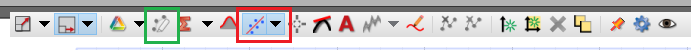
\includegraphics[width=0.9 \linewidth]{lab2-interface-graph-tools}
\caption{Graphing toolbar. The toolbar appears when moving the mouse to the top of the graph. The red boxed icon is the Curve fitting tool. Select the ``Natural Exponential" function. 
The highlighting tool is boxed in green. This allows to select a smaller subset of data to apply the curve fitting.}
\label{Fig:lab2-interface-graph}
\end{figure}

Use this to fit an exponential curve to the discharging region, and {\color{blue} record the value of the parameter $B$ and the order of magnitude of the standard deviation}.

\item {\color{blue} Compare the time constants obtained from both the charging and discharging regions. 
Can you explain the difference in order of magnitude between the standard deviation of the charging versus the discharging measurements?
Calculate the theoretical time constant based on the known values of resistance and capacitance.} 
You can repeat steps 6-10 for different segments of charging/discharging in your data if you want to verify the consistency of your measurements.

\item {\color{blue}Answer the following questions in the results section of your log book.}  Should all the time constants be the same or different? Why and why not? 
What would happen if we had used the rheostat instead of the $470\Omega$ resistor in Fig.~\ref{Fig:lab2-session1-circuit1} and used a DC voltage source (with the On/Off switch on the board) instead of a wavefunction source: would we have the same time constant for both charging and discharging? 
If you have time, you should test your hypotheses experimentally.

\item {\color{blue}Answer the following in the results section of your log book. }
Assuming the voltage, when completely charged, is set to $V_0 = 1$ and by considering the variables $\tau$ for time constant and $t$ for time, what are the equations for of charging and discharging? 
Support your answer by physical arguments.

\item {\color{blue}Answer the following in the results section of your log book.} Your draft calculations can be shown in the ``General Notes" section of the log book. 
In the circuit of Fig.~\ref{Fig:lab2-session1-Rpractice}, how will the fully charged capacitor affect the current and potential in R6? Answer this in your log book.
\begin{figure}[h]
\centering
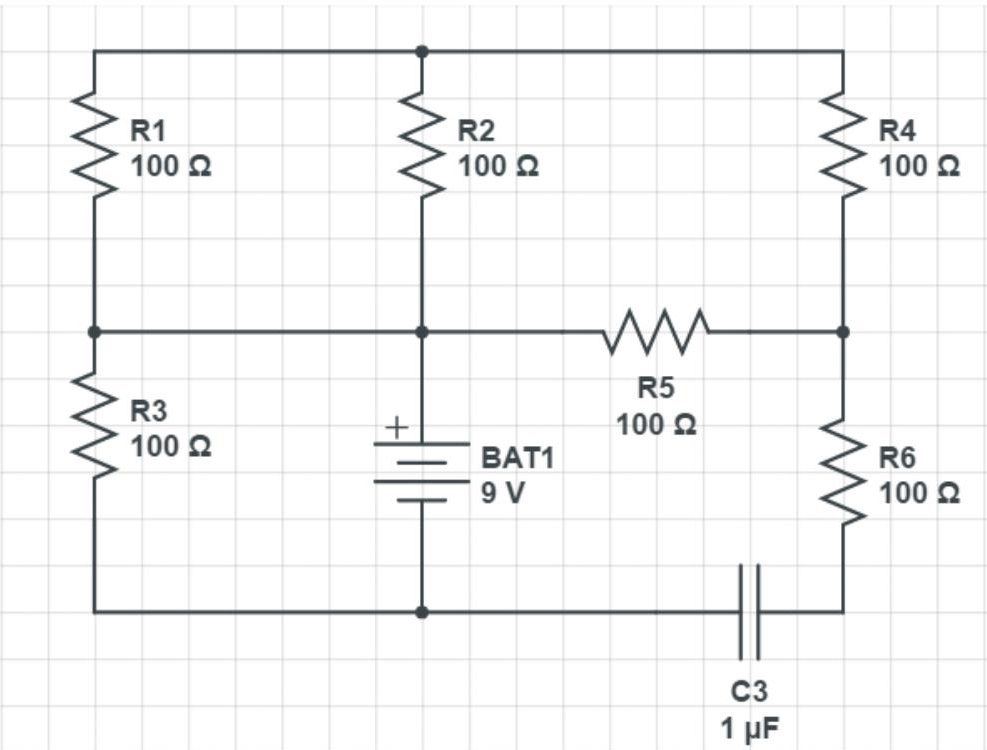
\includegraphics[width=0.6\linewidth]{lab2-session1-Rpractice}
\caption{Effect of a fully charged capacitor on the circuit.}
\label{Fig:lab2-session1-Rpractice}
\end{figure}

\item {\color{blue}Answer the following in the results section of your log book.} Your draft calculations can be shown in the ``General Notes" section of the log book. Given Fig.~\ref{Fig:lab2-session1-tau-practice}, what must be the value of C2 such that the time constant of the equivalent circuit is approximately $\tau=12.5$ms?
If one replaces C2 by two capacitors in series, one of which has $C5=250\mu$F. What must be the capacitance of the second capacitor to preserve the same time constant?
\begin{figure}[h]
\centering
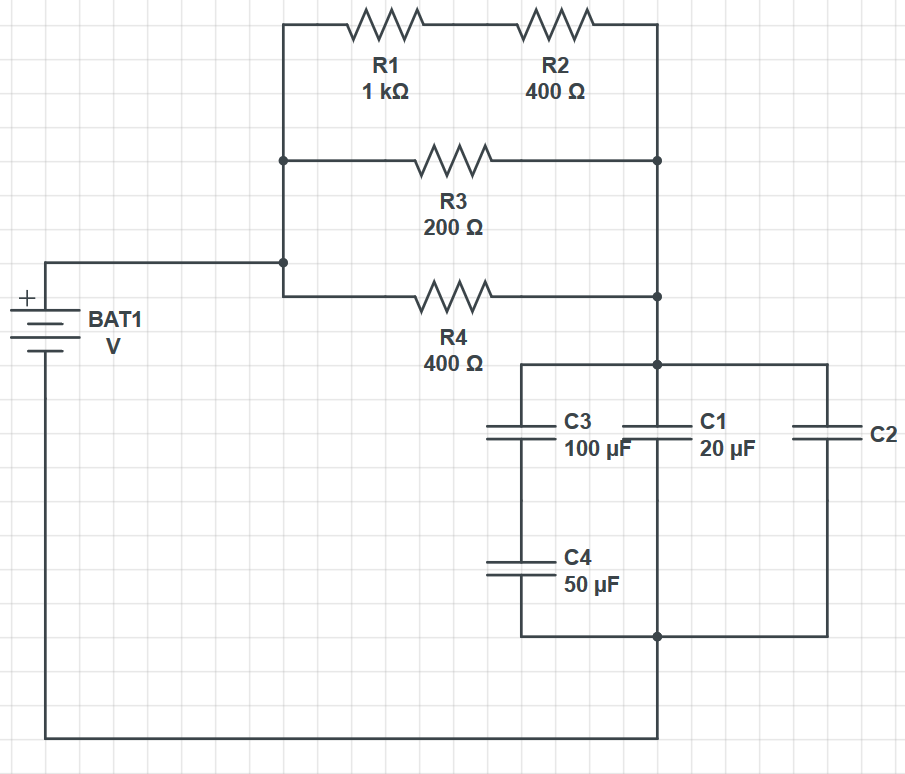
\includegraphics[width=0.6\linewidth]{lab2-session1-Cpractice}
\caption{Time constant practice.}
\label{Fig:lab2-session1-tau-practice}
\end{figure}

\item If you want to keep a trace of a graph produced by the PASCO, click on the Final results tab and select which graph you want by choosing the right run in the scrolling menu of the colored triangle. 
Click on the camera icon on the top panel. This will take a picture that will be accessible in the journal, on the right hand side, where it can be saved as jpeg or html. 
Alternatively, you can also save your whole set of measurements by going to the top left tab ``File", and select ``Save As".
\end{enumerate}

Note: as you step through he above manipulations, make sure to record important technicalities of the time constant measuring methodology in order to accelerate your data acquisition process for the next session. 
You should perform any further tests that you believe would help you better understand the RC circuit in preparation for the next session.

Resistors and capacitors can be found in the lab. Instructions about reading the resistance color-code for resistors can be found in the Appendix.
We recommend that you try and read the resistance of a few resistors and confirm by using the in-lab multimeters. 
An example circuit board that you will use during the next session will be available for you to contemplate. 
We recommend that you observe the set up of the circuit board and think about how you would connect the resistors and capacitors to obtain different equivalent resistance and capacitance setup.

\section{Session b}
In this session, you are asked to build an RC circuit with a specific time constant. When you enter the lab, each station will receive a unique circuit design and a given time constant. 
Your circuit will have two sub-circuits: one that consists only of resistors and another one that consists only of capacitors. 
You are to place both of these in series with the PASCO source as shown in Fig.~\ref{Fig:lab2-session2-circuit}.

\begin{figure}[h]
\centering
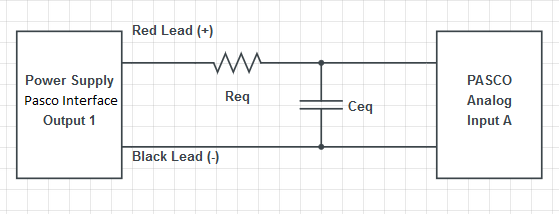
\includegraphics[width=0.9\linewidth]{lab2-session2-circuit}
\caption{RC Circuit. You are to assemble sub-circuits that produces an equivalent resistance $R_{eq}$ and capacitance $C_{eq}$, in such a way as to obtain a desired time constant of the equivalent circuit.}
\label{Fig:lab2-session2-circuit}
\end{figure}

You will only use the ``Positive Square Wave" input for this lab. 
Adjust the frequency and amplitude settings accordingly to your calculated theoretical time constant for each measurement. 
Sometimes, the data fitting tool cannot give standard deviations: this is because the data acquisition frequency isn't properly set. 
Modify the frequency setting until the PASCO's fit function gives an uncertainty for the $B$ parameter. 

There will be a few communal multimeters that allow you to measure capacitance, while every team will have their own multimeter that can only measure resistance. 
There will also be boxes containing different resistors and capacitors. Their values will be labelled but you can double-check their values using the multimeters. 
Note that we are using so-called {\it polarized} capacitors and therefore you must be careful when connecting them to the circuit: the voltage input must be attached to a specific leg of the capacitor. If not the capacitor might explode. If you are unsure, ask the TAs for help. 

While every team will have to build a different RC circuit, the time constants that we are asking are of the order of ms, and therefore you will have to use the "Positive Square Wave" input from the signal generator. 
You have the liberty to choose different values of frequency depending on your estimate time constant. 
Changing the frequency of the input source does not change the time constant: this only changes the duration that the source is "turned on".

%\anhkhoi{Should we tell them the two methods to confirm their measurements? Or should the TAs talk them through it to find the second way?}
%
%To confirm your time constant measurement, you should take two approaches. The first is to simply perform charging and discharging measurements multiple times and average the given time constant measurements.
%
%The second is to confirm your equivalent resistance and capacitance by varying time constant. Since the time constant is $\tau = RC$, if one varies the value of one of the parameters $R$ or $C$ and plot $\tau$ as a function of the varying parameter, one expects the data to show a linear trend where the slope is the value of the other parameter. By performing this test, you will firstly verify eq.\eqref{Eq:time-constant}. Furthermore, this is a complementary method to measure your effective resistance and capacitance which should match your measurements obtained by using the multimeter.

%To accelerate this measurement method,
Each team will have 5 capacitors of $10\pm 1\mu$F and 5 resistors of $50\pm 1 \ \Omega$ from which to construct equivalent resistors and capacitors in their circuits. Since there is a limited quantity of multimeters that can measure capacitance, you can assume that these standard deviations are correct.
A summary of the equipment for this session is shown in Table~\ref{Tab:Lab2-material}.
\begin{table}[h]
\centering
\begin{tabular}{||c | c ||}
\hline
Individual station & Collective station\\ \hline
Laptop & Assorted resistors \\
PASCO 850 interface & Assorted capacitors \\
Resistance multimeter & Capacitance multimeter \\
Resistance and capacitance sub-circuit setups & \\
Five $10\pm 1 \mu$F capacitors & \\
Five $50 \pm 1 \ \Omega$ resistors &  \\
\hline
\end{tabular}
\caption{Available material for Lab \# 2}
\label{Tab:Lab2-material}
\end{table}

{\color{blue}The goal of this lab is for you to \textit{demonstrate} that you've constructed the right RC circuit with the required time constant. 
You should discuss among yourselves and the TAs in order to find appropriate tests to support your claim.}

{\color{blue}Document your results and argue whether or not your RC circuit has the required time constant. If you believe that it does, argue using standard data analysis methods. What is the most appropriate measure to characterize the error of your measurements (see ``Measurement analysis" section of the ``Basic statistics" section)? If your data doesn't produce the correct time constant, explain why. Explain what you must change in your circuit to remedy the situation. Also discuss whether you believe this experiment is adequate to obtain RC time constants. If possible, propose a better way to obtain time constants and/or decrease the error in your experiment.}


\chapter{Lab 3 - Magnetic Field of Solenoids and Coils}
\section{Learning objectives}
\begin{itemize}
\item Learn about solenoids.
\item Learn how to use the right hand rule.
\item Learn about vector nature if magnetic field.
\item Learn about electric motors.
\end{itemize}

\section{Introduction}
The goal of this lab will be to learn about real-world applications of magnetism. In particular, we will study the solenoid in the first session, and build on this to study the electric motor in the second. You will use your data analysis skills previously acquired from the other labs to characterize the magnetic field in these setups.

In the first session, you will be asked to draw the magnetic field lines of the solenoid and to explain your findings in terms of the right hand rule. You will then quantitatively characterize your solenoid's magnetic field. Namely, you will verify the dependence of the magnetic field $B$ of the solenoid on the current $I$ through the solenoid and on the the position $z$ from the end of the solenoid's central axis.

In the second session, having learned how the magnetic field strength of the solenoid varies with distance, you will now use a permanent magnet to construct and characterize an electric motor.

\subsection{Pre-lab activity}
\begin{enumerate}
\item How would you present data that consists of vectors?

\item What is a vector diagram? What needs to be present when drawing a vector diagram?

\item Given the wire below, draw the field lines of the magnetic field generated from the current in the wire.

\begin{figure}[h]
\centering
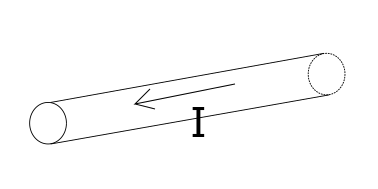
\includegraphics[scale=0.5]{lab3-wire}
\caption{Wire with a current $I$ going from right to left.}
\label{Fig:lab3-prelab-wire}
\end{figure}

\item Does the strength of the magnetic field increase, decrease or is it constant as we go further away from the wire?

\item Imagine stacking multiple wires similar to that of Fig.~\ref{Fig:lab3-prelab-wire} parallel to each other, with the current of each all running in the same direction. Would the magnetic field close to the stack of wires  be greater, equal or smaller than the scenario with a single wire?

\item Given the wire below with a constant magnetic field $B$ pointing downwards, what is the direction of the magnetic force that $B$ exerts on the wire?

\begin{figure}[h]
\centering
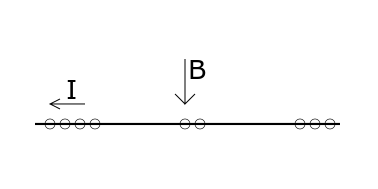
\includegraphics[scale=0.85]{lab3-wire-bfield-force}
\caption{A wire has a current running through it, hence electrons are running from right to left. A constant magnetic field is present and points downwards. The circles are electrons.}
\end{figure}

\end{enumerate}

\section{Session a}
\subsection{Solenoid setup}
In this session, you will use the IOLab that you previously used in PHYS 101 last semester to measure magnetic field strength of a solenoid at different locations around the solenoid.

\begin{figure}[h]
\centering
\begin{subfigure}{0.45 \textwidth}
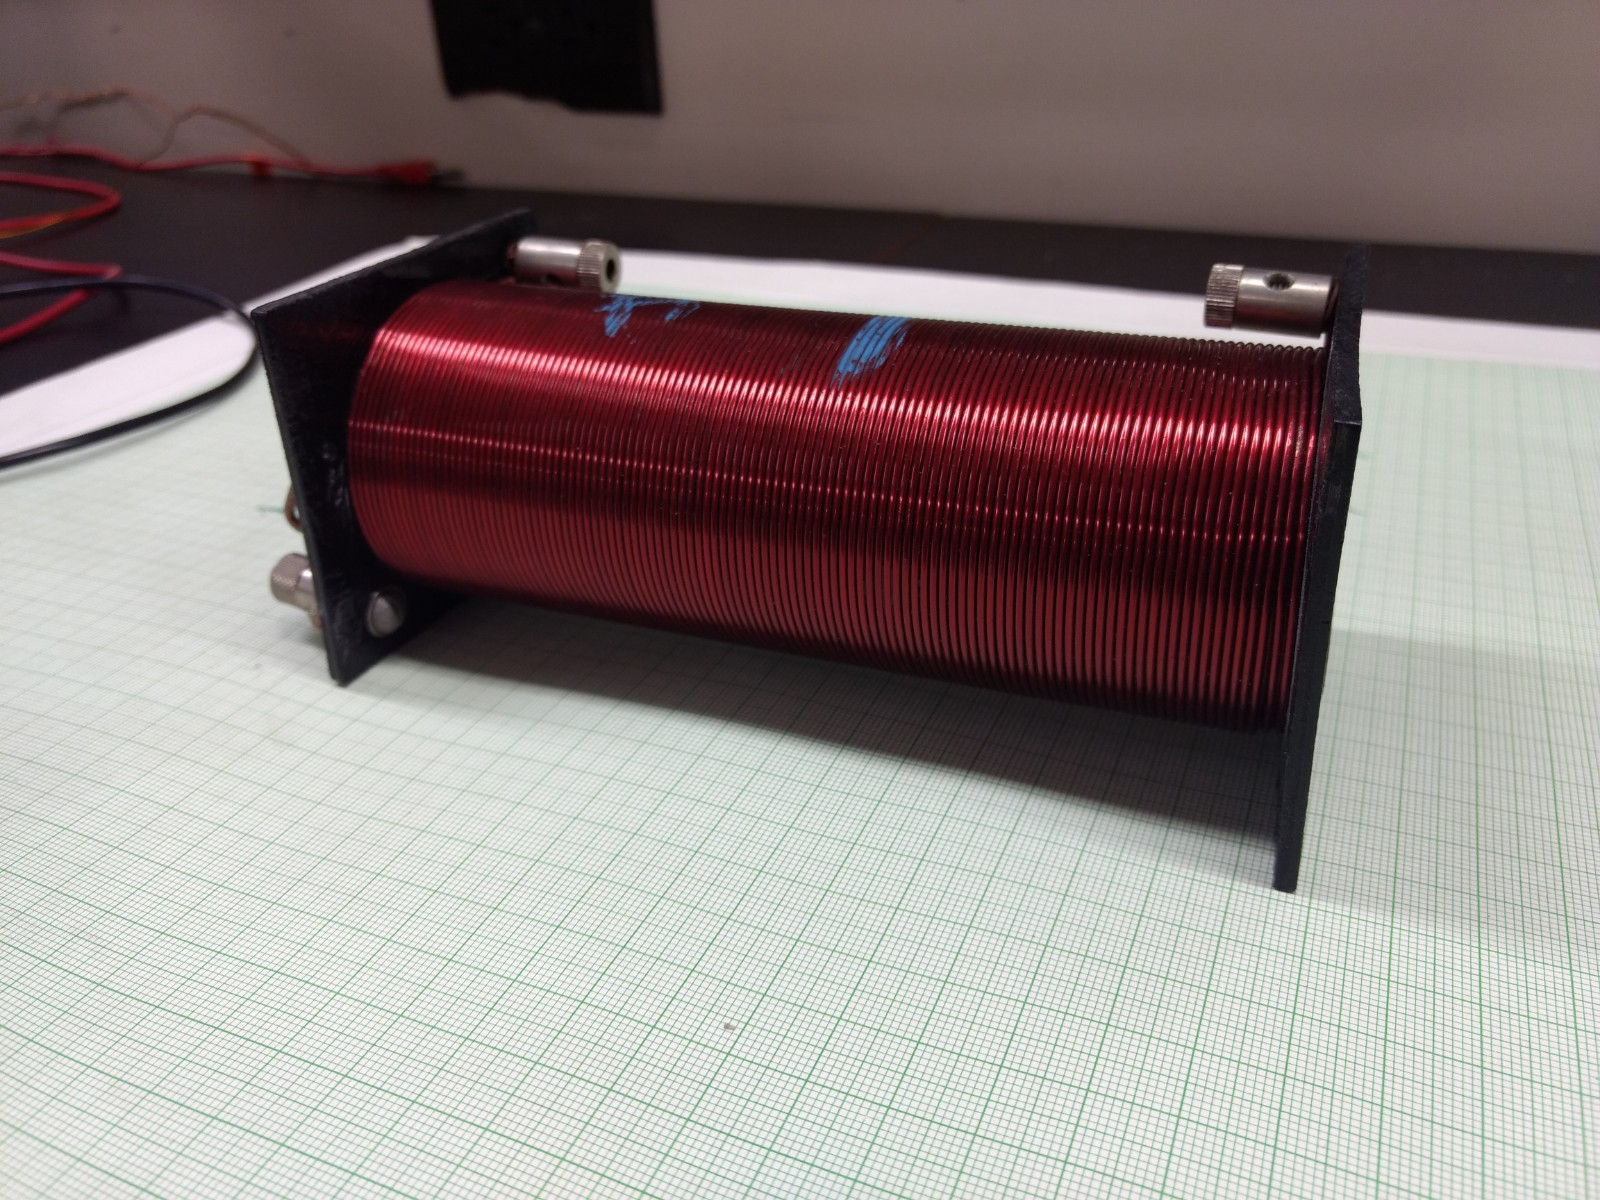
\includegraphics[width=\textwidth]{lab3-sessiona-solenoid1}
\end{subfigure}
\begin{subfigure}{0.45 \textwidth}
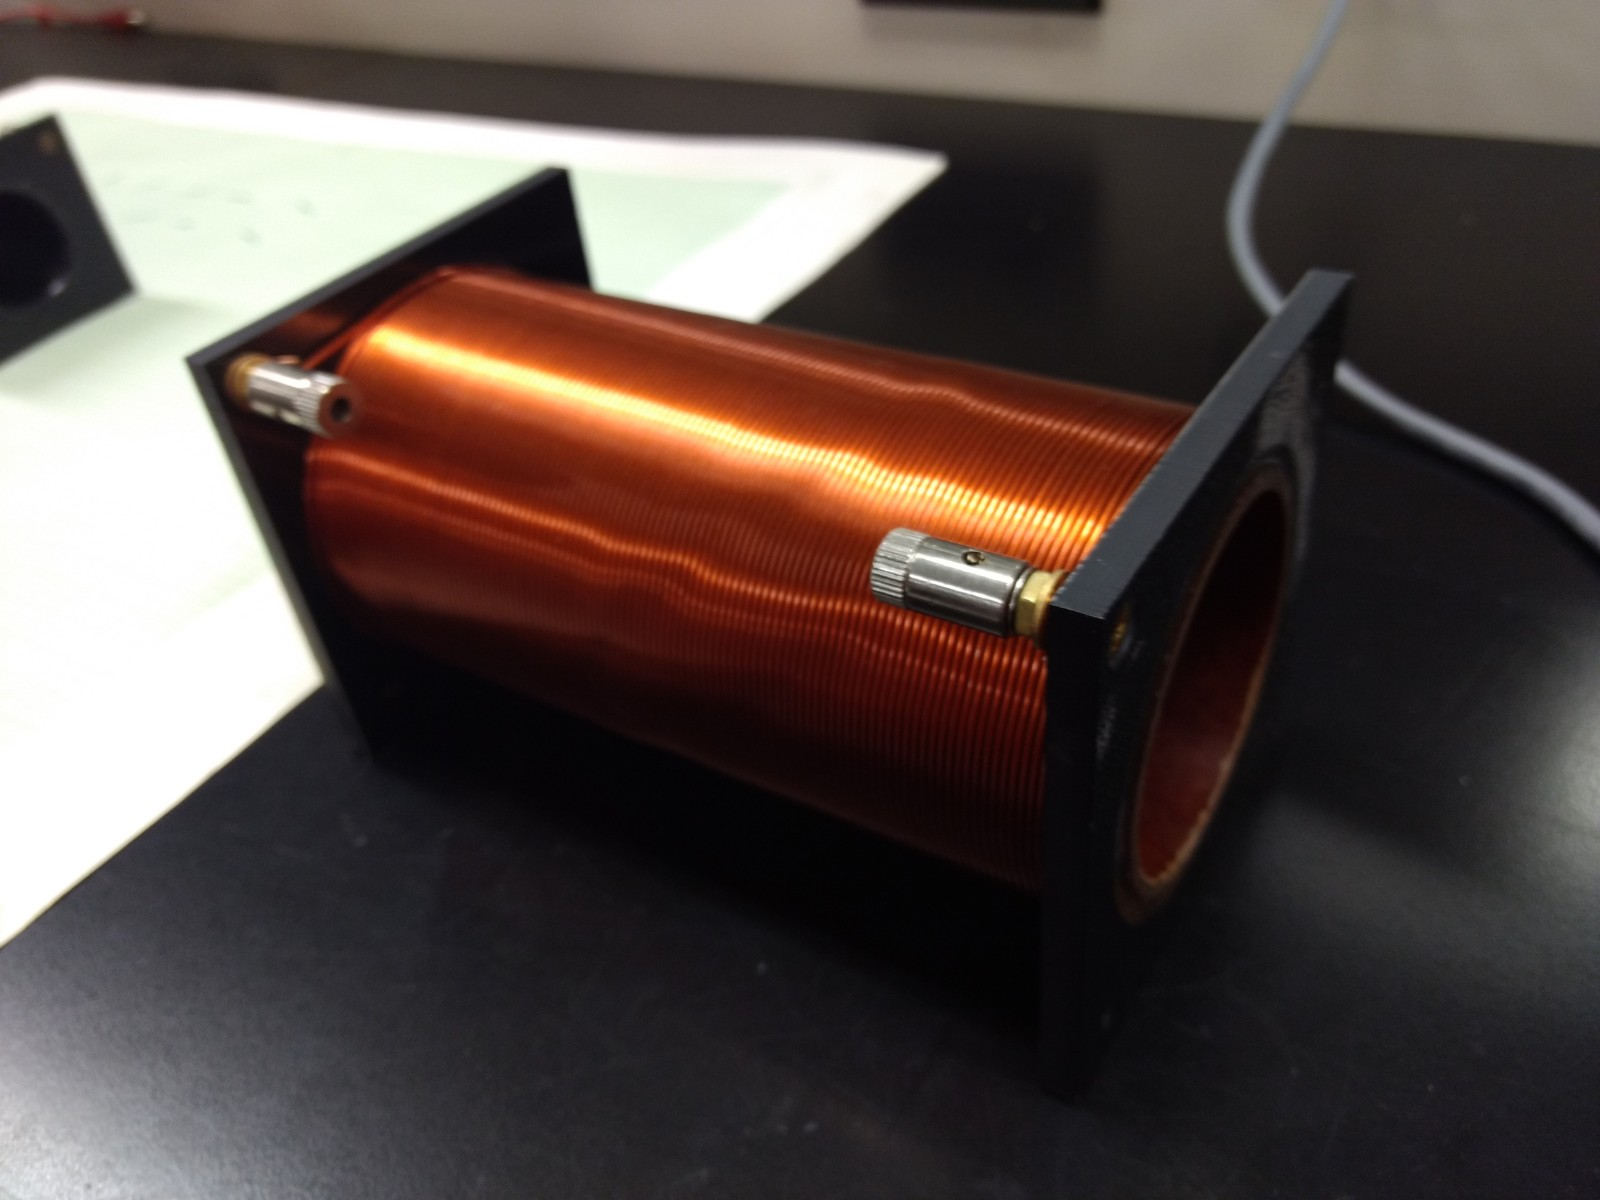
\includegraphics[width=\textwidth]{lab3-sessiona-solenoid2}
\end{subfigure}
\caption{Available solenoids. The one one the left has a smaller radius ($2.25$ cm radius, 550 turns of wire, $15$ cm of length, \#16 gauge wire), while the one on the right is larger ($3$ cm radius, 560 turns and $15$ cm of length, \#19 gauge wire).}
\label{Fig:lab3-sessiona-solenoids}
\end{figure}

Each team will have access to two solenoids as shown in Fig.~\ref{Fig:lab3-sessiona-solenoids}. We will mostly use the one with the smaller radius. You are to connect the two leads to the power supply. This will generate a current through the wire turns.

\begin{figure}[h]
\centering
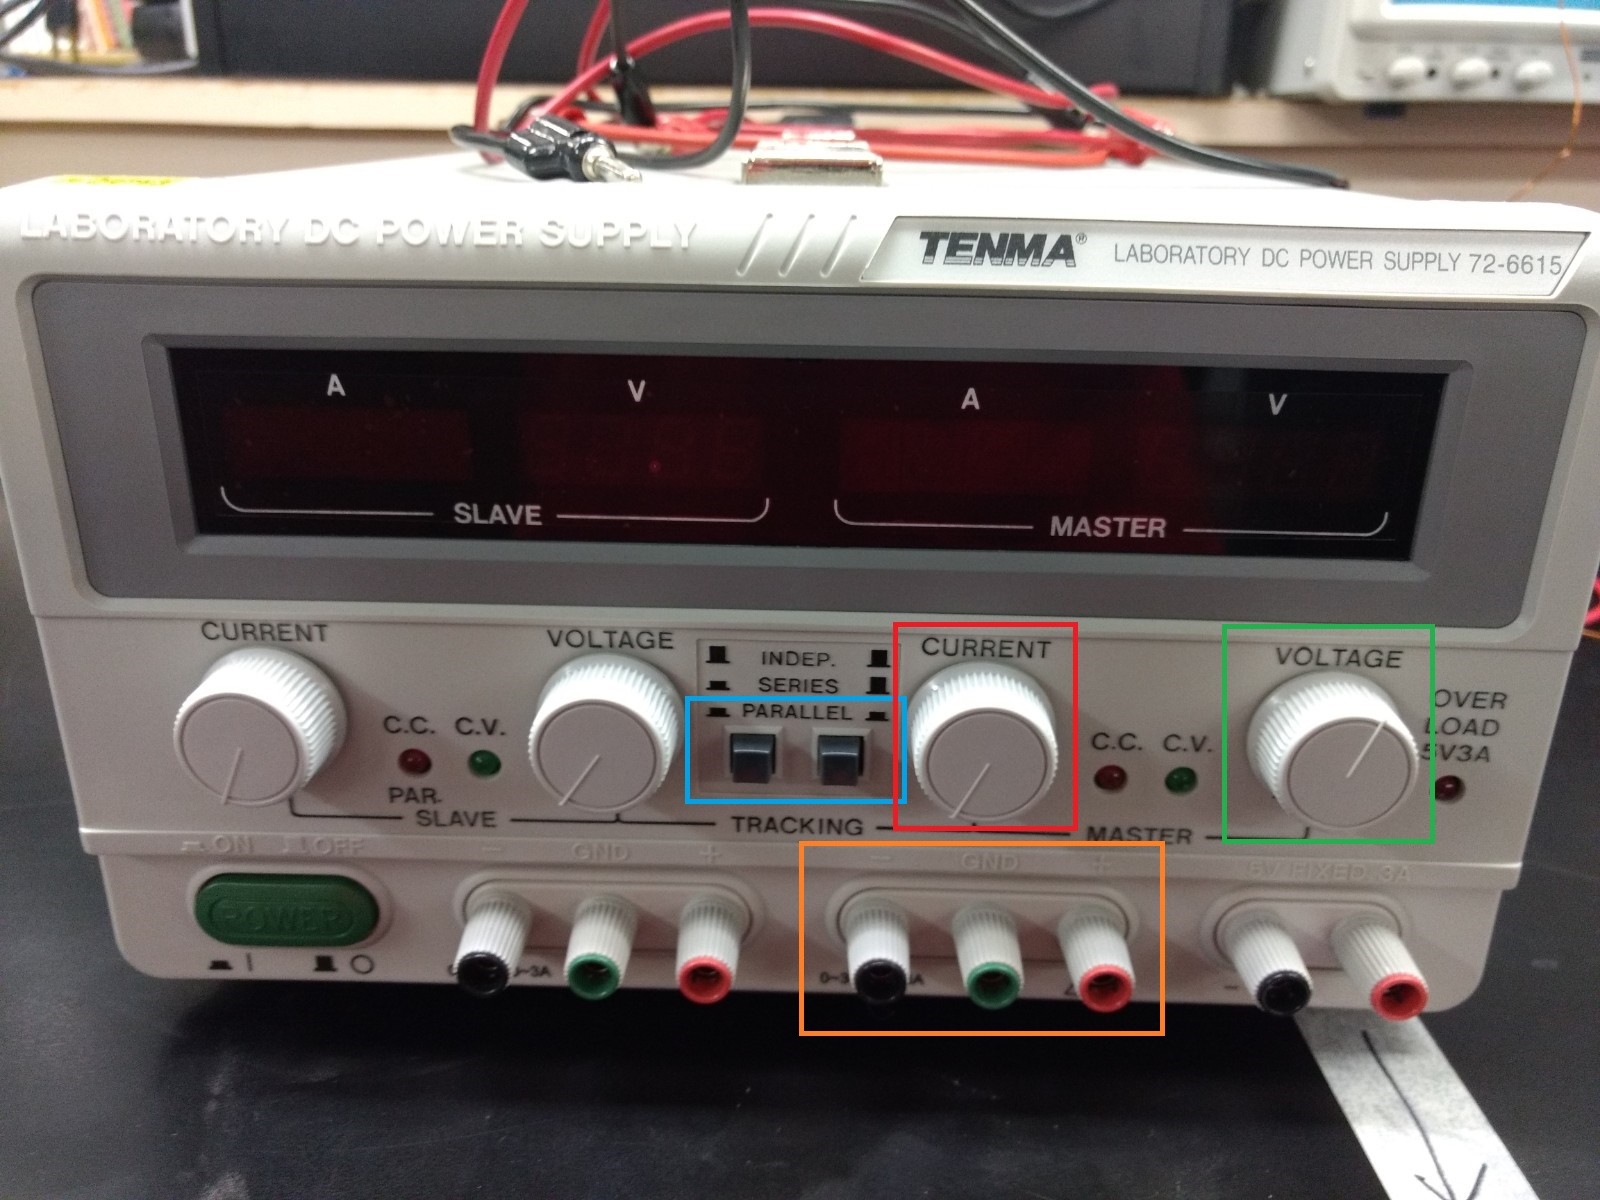
\includegraphics[scale=0.4]{lab3-power-supply}
\caption{Power supply.}
\label{Fig:lab3-power-supply}
\end{figure}
Fig.~\ref{Fig:lab3-power-supply} shows a typical power supply used for this lab. To use the power supply:
\begin{enumerate}
\item Make sure both knobs (red and green box) on the ``master" side are completely turned down.
\item Connect your wires to terminals in the orange box (red for input, black for output).
\item Make sure to press down on both buttons in the blue box so that the power supply is set on ``parallel". This will allow you to go up to 6A of current.
\item Turn the voltage knob to halfway (green box). This sets the maximum amount of voltage allowed.
\item You will control the voltage and current of the power supply by slowly turning the current knob (red box).\\
\end{enumerate}

To measure magnetic field data, you will use the IOLab:
\begin{enumerate}
\item Connect the IOLab USB to your laptop and open the IOLab software.
\item Calibrate your IOLab as shown in Fig.~\ref{Fig:lab3-sessiona-interface1} 

\begin{figure}[h]
\centering
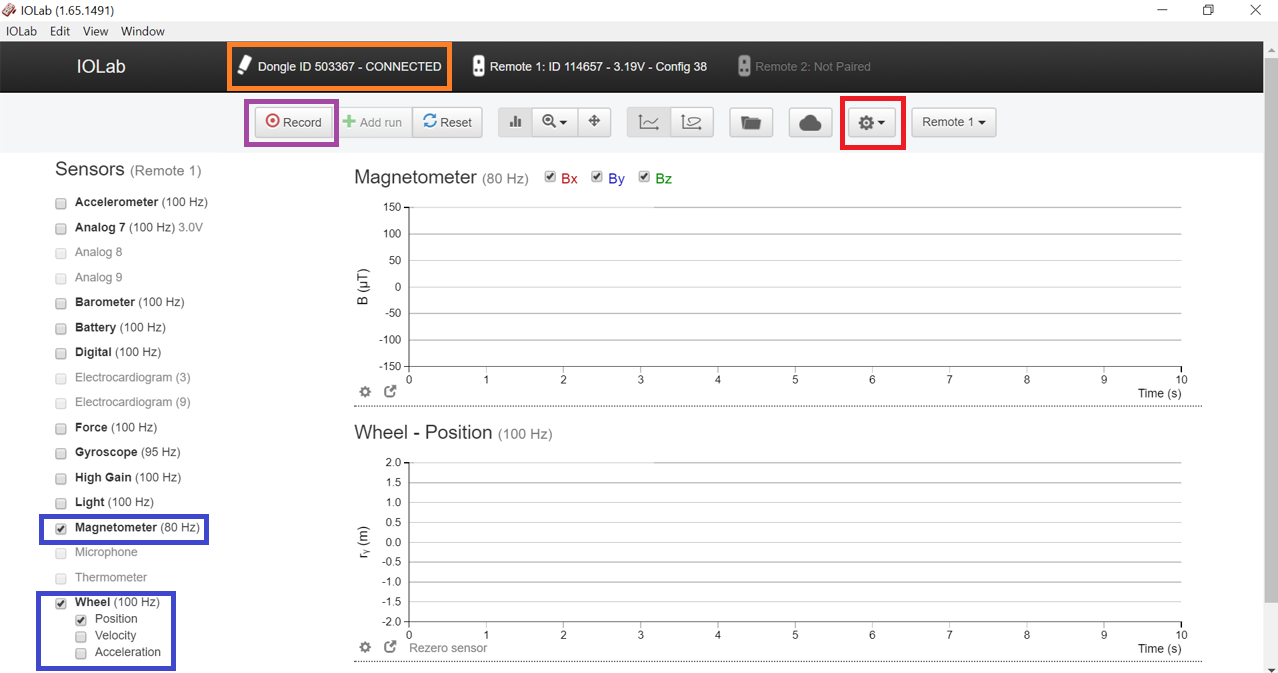
\includegraphics[width=0.8 \textwidth]{lab3-sessiona-interface1}
\caption{IOLab interface. Firstly, make sure the IOLab is connected to the bluetooth USB stick: the area labelled by the orange box should indicate ``Connected". Afterwards, calibrate your IOLab by clicking the button labelled by the red box $\rightarrow$ ``Calibration" $\rightarrow$ ``Remote 1" $\rightarrow$ ``Accel - magn - gyro" and follow the subsequent on-screen instructions. We will use the ``Magnetometer" and ``Wheel" sensors (see blue boxes). When you are ready to make measurements, press the record button (purple box). }
\label{Fig:lab3-sessiona-interface1}
\end{figure}

\item On the left of the interface, select the ``Magnetometer" and ``Wheel" sensors. We will only need the position data, not the velocity or acceleration plots.

\item When you are ready to acquire data, you can start recording by clicking the record button. The data should appear as in Fig.~\ref{Fig:lab3-sessiona-iolab-interface2}.
\end{enumerate}

\begin{figure}[h]
\centering
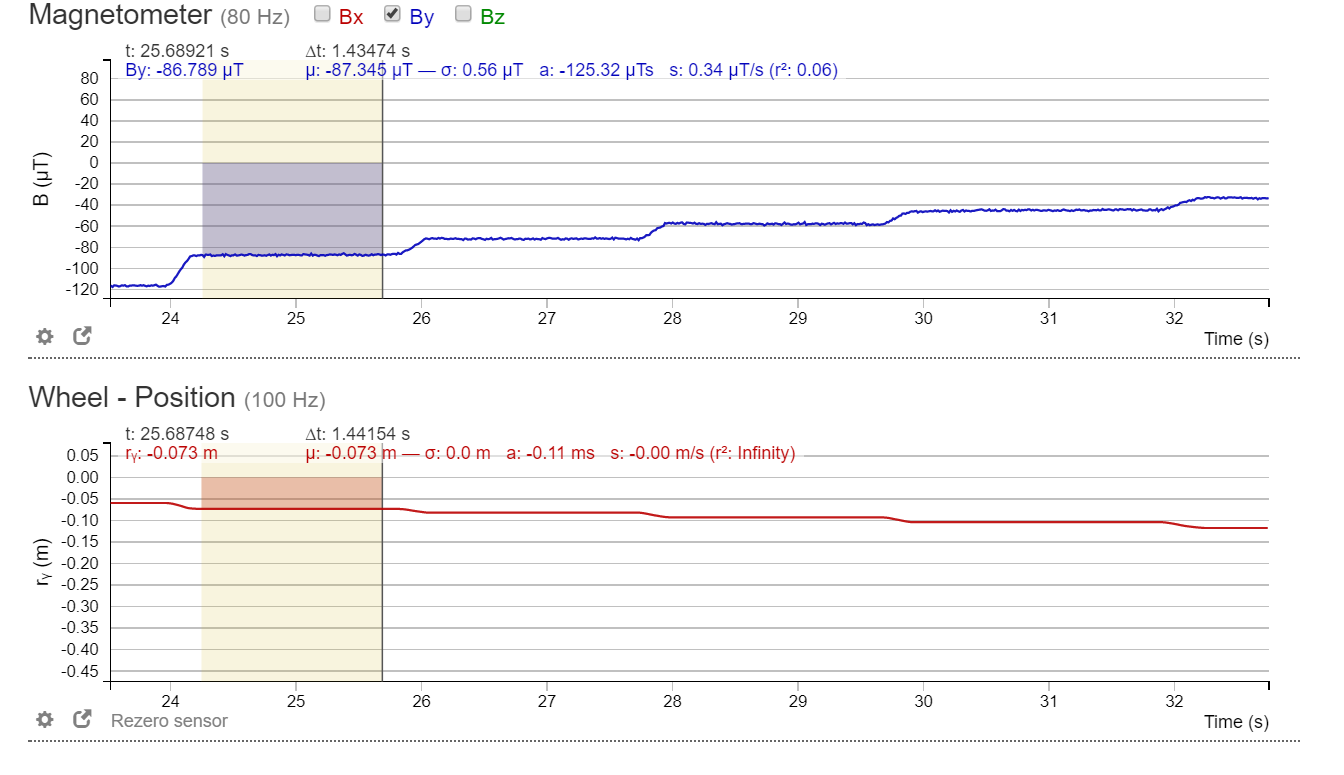
\includegraphics[width=0.8\textwidth]{iolab-data-selection.PNG}
\caption{Data sample. You can select an interval of your data. Doing so, you can obtain directly the average ($\mu$) and the standard deviation ($\sigma$) of your data within that interval. For this lab, you should move the IOLab to a desired position, and wait a few seconds before moving it again. This way, you can obtain an average value of the magnetic field at that position. In the figure above you see a plateau, its size depends on the amount of time you left the IOLab at each position. You should only average the magnetic field during each of the plateaus to make sure you are not registering data at intermediate positions. By doing this incrementally, your data should look like a staircase as a function of time.}
\label{Fig:lab3-sessiona-iolab-interface2}
\end{figure}

The protocol is straightforward: you will move the IOLab to a given position and observe the magnetic field strength at that position. Leave the IOLab at that position for a few seconds so that you can select that interval in your data to obtain the standard deviation ($\sigma$) and mean ($\mu$) of that measurement (See Fig.~\ref{Fig:lab3-sessiona-iolab-interface2}). Repeat the above for all the positions that you wish to measure the magnetic field.

Further details about the IOLab can be found in the appendix.

\subsection{Magnetic Field Lines}
Once the solenoid has been properly connected, you are asked to draw field lines on the graph paper on which the solenoid is placed as shown in Fig.~\ref{Fig:lab3-sessiona-solenoids}. For this, we will use the compass and IOLab. Place the compass on top of the sensor. Note that the magnetometer isn't centered in the IOLab; the magnetometer sensor of the IOLab is located in one of the corners of the device as shown in Fig.~\ref{Fig:lab3-sessiona-iolab-sensor}.

\begin{figure}[h]
\centering
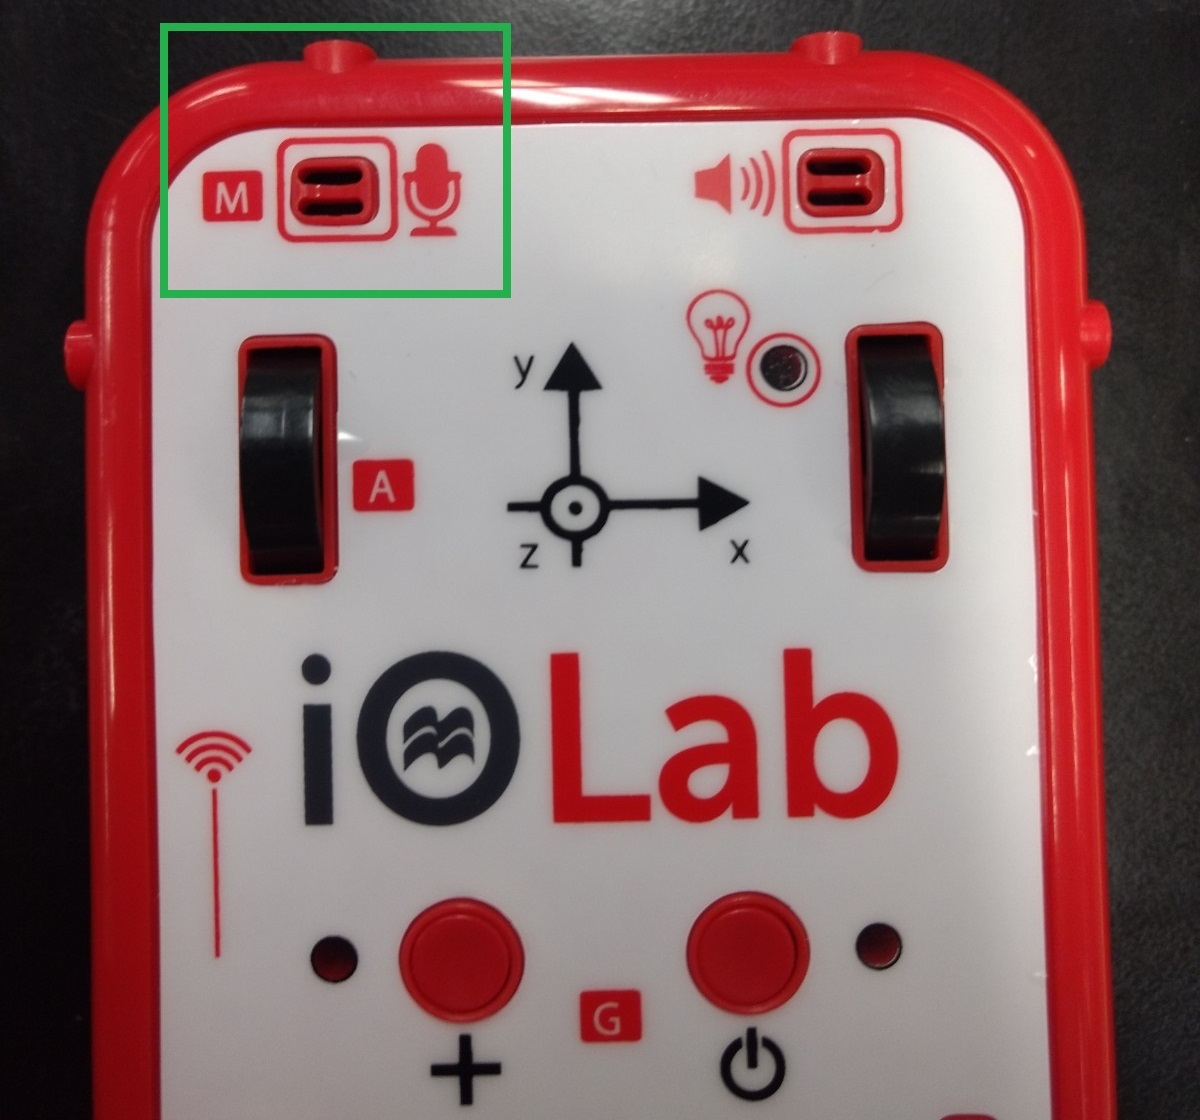
\includegraphics[scale=0.3]{lab3-sessiona-iolab-sensor}
\caption{Position of the magnetometer on the IOLab (green box). Place the compass on top at this position to obtain precisely the direction of the magnetic field detected by the IOLab.}
\label{Fig:lab3-sessiona-iolab-sensor}
\end{figure}

First, chose at least a dozen points on the graph paper to place the IOLab. For each point, you are to measure the orientation of the magnetic field with the compass, draw a vector arrow associated with your observation, and write next to the vector the measured strength of the the magnetic field. Recall that the total magnitude of the magnetic field will be given by Pythagoras' theorem:
\begin{equation}
| \mathbf{B} | = \sqrt{B_x^2 +B_y^2}.
\end{equation}
Both vector components can be obtained from the IOLab (see Fig.~\ref{Fig:lab3-sessiona-iolab-interface2}). Normally, one would draw the length of the vector to represent the magnitude of the vector, however for the amount of vector lines you are asked to draw, we will simply write the magnitude next to the drawn vector.

Once you have measured $\mathbf{B}$ of the solenoid at enough points, and have explored the possible orientations of the magnetic field vector lines, {\color{blue}answer the following questions in the General Notes Section of your log book:}
\begin{enumerate}
\item Draw a diagram of the solenoid with the appropriate field lines surrounding it.

\item What is the behaviour of the magnetic field inside the solenoid? Support your claim of the field lines inside the solenoid in terms of the right hand rule.
\item What happens if you swap the connections of the solenoid? What would change? Explain this in terms of the right hand rule.
\item Do these field lines look like any other magnetic object that you've seen? Explain why this observation is true.

\item What parameters do you expect to affect the strength of the magnetic field of the solenoid? Give a brief explanation for each parameter.

\end{enumerate}

\subsection{Current dependence}
Now that you have a qualitative idea how a solenoid generates a magnetic field, we will quantitatively verify its dependence on some of the possible parameters of this set up.

We will first verify the $B$ dependence of the solenoid on the current through the wires. Place the IOLab on the ramp at a fixed distance away from one end of the solenoid (not too far) as shown in Fig.~\ref{Fig:lab3-sessiona-ramp}, and increase the current through the wires with the power supply. 

\begin{figure}[h]
\centering
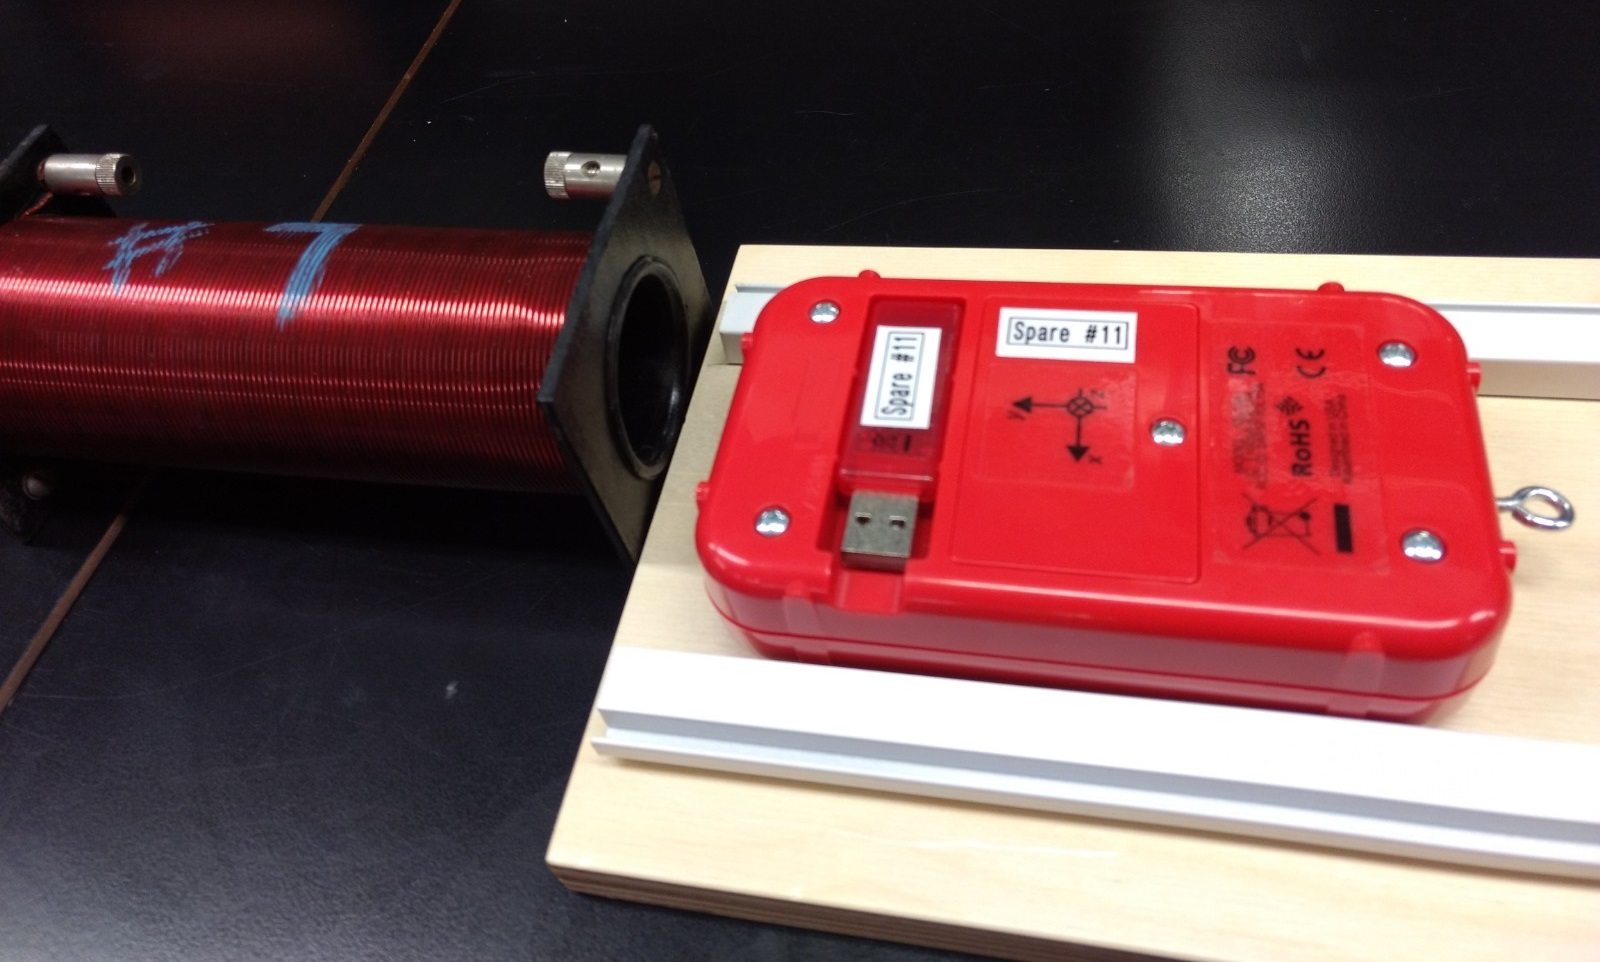
\includegraphics[width=0.8\textwidth]{lab3-sessiona-ramp}
\caption{Measuring the distance dependence of the magnetic field. Place the ramp in front of the solenoid and use it as a guide for moving the IOLab.}
\label{Fig:lab3-sessiona-ramp}
\end{figure}

{\color{blue}Verify how $\mathbf{B}$ depends on $I$ using your data analysis skills from previous labs. Find the parametric dependence on the current $I$ and carefully support your claim by generating a graph with an appropriate fit and error analysis.
Recall that you are not evaluated on the rigorous standards of \textbf{data presentation} during this session, however you should perform an appropriate analysis to be confidant in your data. }

\subsection{Distance dependence}
We will now verify the magnetic field generated by a solenoid at a distance $z$ (on the central axis) away from the front of the solenoid.

Place the ramp in front of the solenoid such that the IOLab sensor is centred in front the solenoid (see Fig.~\ref{Fig:lab3-sessiona-ramp}). 
Recall that the sensor isn't centered. Move the IOLab incrementally, and {\color{blue}at each position, use the interface in order to obtain the average and standard deviation of the position and magnetic field of the measurement. }
You will not need to go further than 30 cm. We recommend that you perform multiple trials to obtain many data points.

Once you have data for the magnetic field for numerous positions $z<30$cm, we will first restrict our analysis to the behaviour of $\mathbf{B}$ at large distances $z$. It turns out that the $B$ field should follow a $1/z^3$ behaviour as $z$ moves far from the centre of the solenoid. 
{\color{blue}Select appropriate data points that are far enough away (called the "far $z$" region) such that you see a good $1/z^3$ fit. Can you explain the minimum value of $z$ for which you performed a cutoff in your data?} You may perform this analysis again with the other solenoid if you wish.



%Once you have obtained data for the far behavior, the TAs will write the equation of the magnetic field of a solenoid on the board and you are asked to compare the intermediate regime to this equation: write the equation in Excel and compare your plots with your data.

{\color{blue} Why do you think that we find a $1/z^3$ behaviour far away?
Why doesn't this fit work for other regimes of $z$?
Can you compare the $1/z^3$ behaviour to other electromagnetic systems that you may know: the electric field of a point charge, the magnetic field from a line
%, a plane wave
?}
%Does your data match the equation on the board? What about the far $z$ behaviour? Why is it useful to restrict to the far $z$ regime? Discuss your results.

\section{Session b}
\Large{\textbf{WARNING!}} \normalsize The permanent magnets used in this experiment are quite strong. Avoid bringing any objects that are magnetizable (made of iron/steel/Ni/Co, ID /credit cards)  near the magnets. \textbf{Students with pacemakers could be excused from this lab.} \\

In this session, we will study the electric motor. The electric motor is a device that converts electrical energy into mechanical energy. Electric motors and their counter-parts, electric generators, have been around for decades now and have become so ubiquitous in our daily lives that life without them would seem almost impossible. Over the years, these motors have grown in complexity and sophistication in order to perform a number of different tasks but the basic physical principles behind their operation have not changed.

The goal of this lab is to provide a general understanding of how a simple DC motor works with the hope that it might lead to a better appreciation for the more sophisticated devices found all around us. This lab is not ``complicated" to do, but will require a number of different concepts in electricity, magnetism and circuit theory to complete.

The main observable of this lab is the frequency of rotation $f$ of the motor.
In class, you've seen how torque can be generated on a loop carrying current. {\color{blue} Explain how physically the frequency of rotation that you are observing is related to the torque.} In fact, the torque is proportional to the frequency of rotation.
Similar to the first capacitance lab, you are also asked to find possible parameters that could affect the frequency of rotation of the motor.

\subsection{Electric motor setup}
For this lab, you are given a power supply, a digital oscilloscope, an electric motor and a magnet. 
Fig.~\ref{Fig:lab3-sessionb-diagram} shows the schematic diagram of the setup we will use in this experiment and Fig.~\ref{Fig:lab3-sessionb-setup} shows a photograph of the actual setup. 

\begin{figure}[h]
\centering
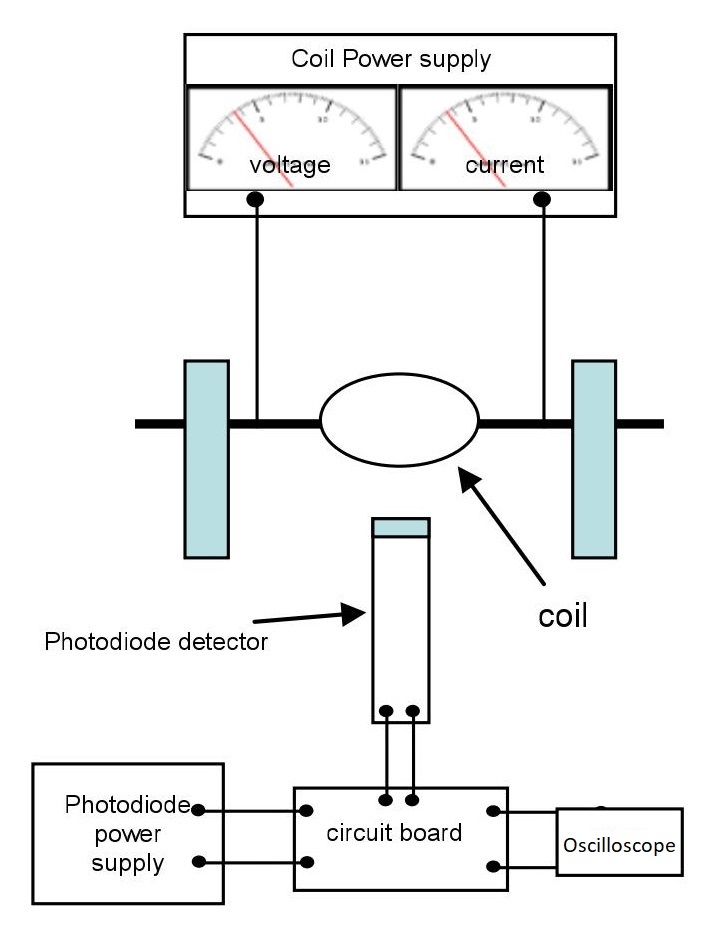
\includegraphics[scale=1.1]{lab3-sessionb-diagram}
\caption{Circuit diagram of the setup (front view)}
\label{Fig:lab3-sessionb-diagram}
\end{figure}

\begin{figure}[h]
\centering
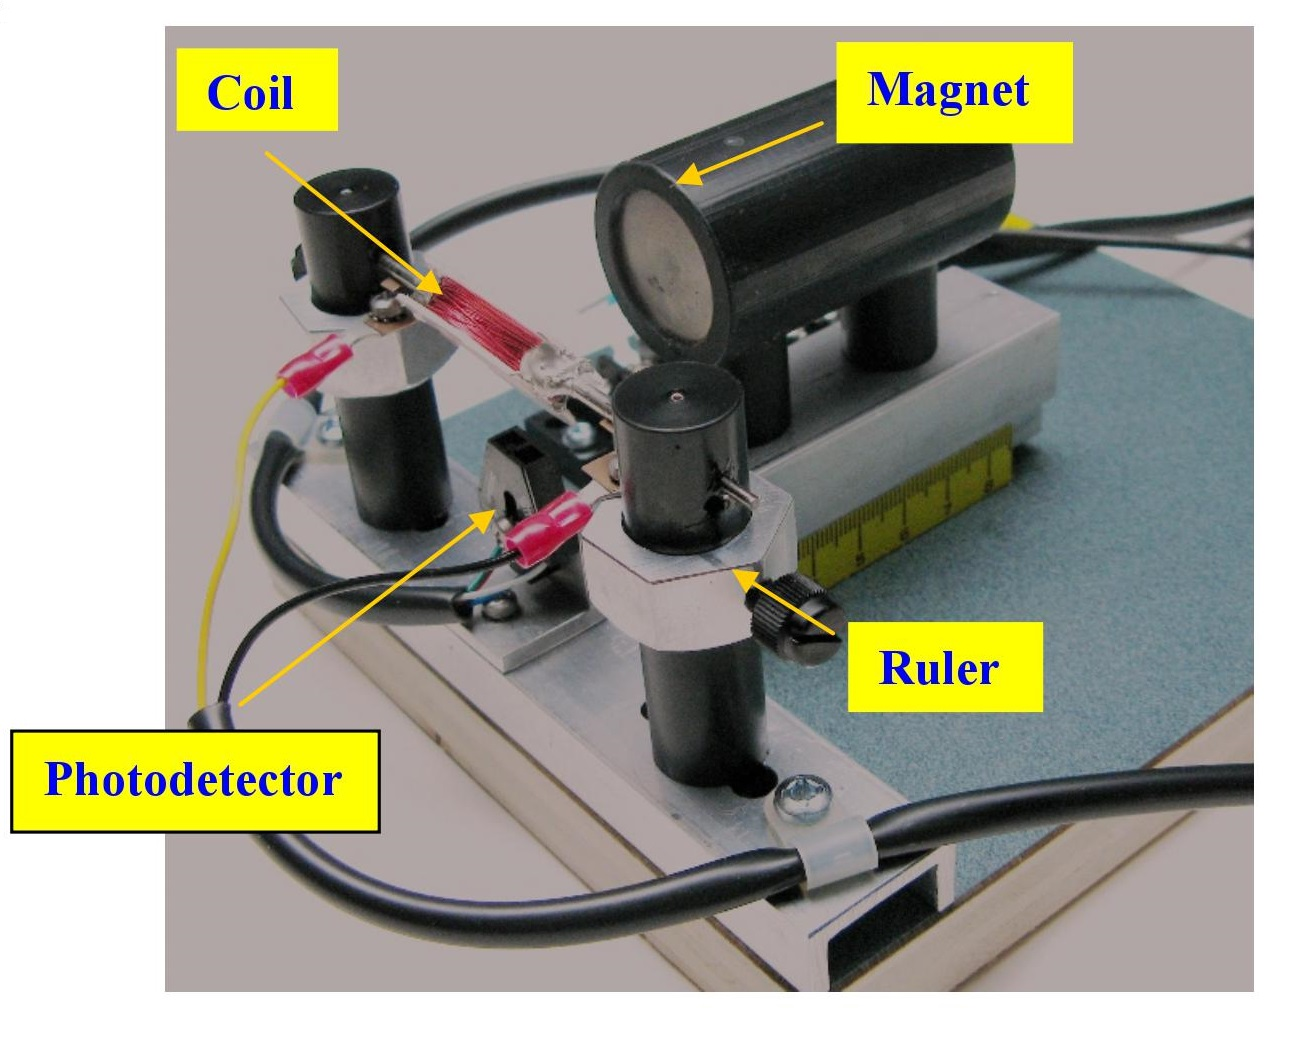
\includegraphics[scale=0.9]{lab3-sessionb-setup}
\caption{Photograph of the setup (Oscilloscope and power supply out of the picture range.)}
\label{Fig:lab3-sessionb-setup}
\end{figure}

To set up the apparatus:
\begin{itemize}
\item Make sure the power supply is turned off
\item Connect the leads from the coil to the power supply.
\item See the instructions for the oscilloscope in the appendix.
\end{itemize}

The coil current and the voltage will be read from the power supply meters. The coil's period of rotation will be measured by a photodiode detector connected to a digital oscilloscope. The photodiode emits light and detects its reflection from the shiny strip covering one side of the coil. The other side is covered by a non-reflective strip. When the coil is rotating, a signal/pulse will be seen on the oscilloscope screen every time the reflected light strikes the detector. The period will be the time interval between two reflected signals/pulses. From the period you can calculate the frequency. 

The performance of the motor and preciseness of measurements are extremely sensitive to the positions of the photodiode and brushes. \textbf{Please be careful with the apparatus, and do not make any adjustments from how it was set up.}

In addition to the electric motor, you are given a magnet that can move on a track. 
Figure~\ref{Fig:lab3-sessionb-calibration-bfield} below is a calibration of the magnet. This should remind you of your data in the last session. \\

\begin{figure}[h]
\centering
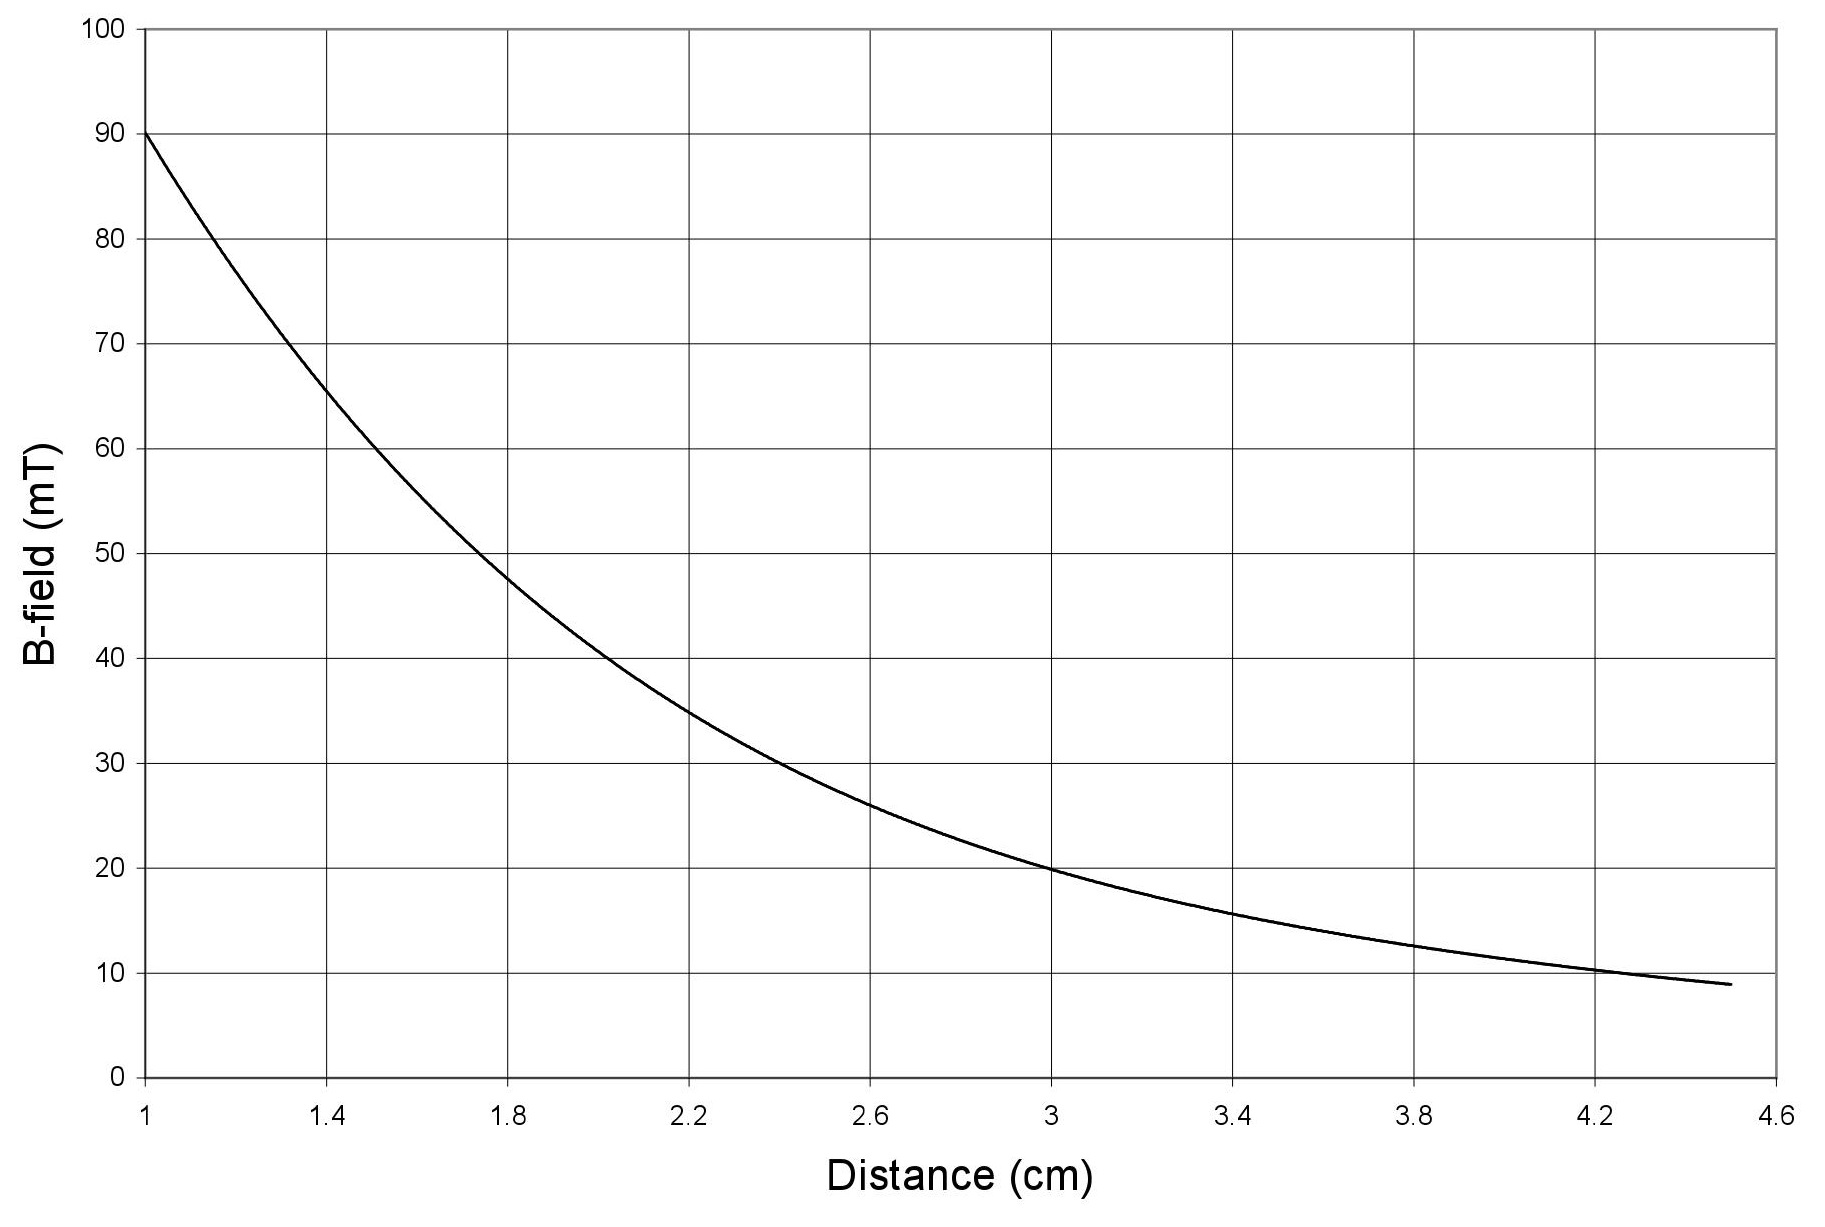
\includegraphics[scale=0.8]{lab3-sessionb-calibration-bfield}
\caption{$\mathbf{B}$ field as a function of distance from the face of the magnet.}
\label{Fig:lab3-sessionb-calibration-bfield}
\end{figure}

%In the previous lab, you showed found that on its axis, the magnetic field generated by a solenoid decreases by a function similar to Fig.~\ref{}. In this figure, we are giving you the calibration of the magnetic field of the magnet as a function of position. You can use this to determine the strength of the magnetic field on the coil at a given distance.\\

\large \textbf{Please respect the following instructions in order to avoid damaging the apparatus:} \normalsize
\begin{itemize}
\item Do not exceed a voltage of 10 V. Do not add the voltages in the slave and master display.
\item Do not let the magnet be any closer than 1 cm to the coils.
\item It may happen that for a large enough voltage and close enough distance, the magnet might vibrate or be pulled towards the coils. Do not let it be any closer than 1 cm to the coils! Hold your magnet in place if necessary.
\item If you are using high voltages (greater than 8 V), try to move quickly through the higher voltages to reduce wear on the brushes.
\item Remember to turn off the power supply after you have finished all your measurements.
\end{itemize}


\subsection{Protocol}
In this lab, you will find what parameters affect the frequency of rotation of the motor $f$. The magnetic field driving the motor will be that of a solenoid, and looks like the one you measured in the previous session. It has been pre-tabulated and given in  Fig.~\ref{Fig:lab3-sessionb-calibration-bfield}.

To characterize frequency, recall that you must isolate your system and vary one parameter at a time in order to perform the analysis. As a starting point, we suggest that you draw a force diagram of the coils of the motor (recall magnetic moment from class). Recall your answers from the pre-lab activity.

To make a measurement,
\begin{enumerate}
\item Make sure you read the previous instructions (above) in order to avoid damaging the apparatus.
\item Set the magnet at a desired position (\textbf{greater than 1 cm away from the coils}).
\item Turn the power supply to a desired voltage (\textbf{do not exceed 10 V}).
\item The coil should start to rotate, though you will likely need to flick it gently with your finger to get it started.
\item Measure the period $T$ from the time interval between two successive pulses from the oscilloscope.
\item For better precision, you may count the time interval between a few pulses and divide it by the number of intervals to get a better value for $T$. The frequency will be given by $f = 1/T$. Note the value of $f$ in an Excel sheet as a function of any other relevant parameters you varied in  this measurement. Remember to keep track of errors in your measurements.
\end{enumerate}

{\color{blue} Through performing your measurements, and through discussions with your lab partners, other teams and the TA, establish a (mathematical) relation between possible parameters that could affect the frequency of rotation of the electric motor. 
Support your claims based on data and figures as usual. Record your procedures and record your data, and discuss your rational in your log book.}



\part{Appendix}
\label{Part:Appendix}
\begin{appendix}

%\renewcommand{\chaptername}{Appendix}
%\renewcommand{\thechapter}{\Alph{chapter}}
%\setcounter{chapter}{0}

\chapter{Introduction to Excel}
\label{App:Excel}

These labs will make use of Excel to plot data. There will be a "lab 0"/tutorial session before official labs start to review error analysis and Excel, the latter of which is also summarized in this appendix, which should be brought to Lab 0. Every McGill student can obtain a free copy of Microsoft Office software by clicking \href{http://kb.mcgill.ca/kb/article?ArticleId=5172&source=Article&c=12&cid=2}{here}. Excel spreadsheet boxes can take in strings of letters of numbers as input. If the input is a number, we can easily perform calculations.\\

\noindent \large \textbf{Performing Spreadsheet Calculations} \normalsize
\begin{itemize}
\item To initialize the math environment, simply click on a box, and press the ``=" key on your keyboard. Press ``Enter" when you are done.
\item One can perform basic addition (+), subtraction (-), multiplication (*) and division (/) between two boxes. One can also take powers by using `` ^ " i.e. x^2 would be $x^2$. First, press ``=", click on the box of your first variable, choose one of the above manipulations and choose another box as your second variable.
\item Excel obeys order of operators: multiplication and division come before addition and subtraction. Parentheses are done first.
\item Note that the middle bar above states the equality function in terms of \textit{boxes} of the spreadsheet.
\begin{figure}[h]
\centering
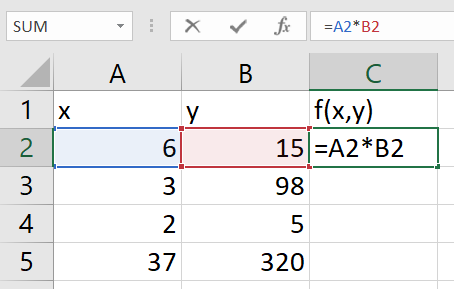
\includegraphics[width=0.4 \textwidth]{Excel-tut-boxes.png}
\caption{Example of multiplication between two variables $x$ and $y$. Notice that the selected box has a green border around which the bottom right corner has an enlarged square.}
\label{Fig:Excel-boxes}
\end{figure}
\item It is useful to separate your data into columns. In this way, say your first two columns are your $x$ and $y$ variables that were obtained from a measurement. You should compute $f(x_i, y_i)$ in another column. Doing so, after performing the mathematical manipulation that you wish, you can click the bottom right green border of a box, and \textit{pull} down to the column to apply the same function along the columns of the input variables. In the example of Fig.~\ref{Fig:Excel-boxes}, one could obtain the multiplication of each element of columns A times those of column B displayed in column C.
\item When defining a function with the intent of dragging the select-box down to apply the whole function to all elements of columns, it is sometimes useful to define a box that \underline{doesn't change} as you drag the select-box. To do so, one uses the \$ sign as in Fig.~\ref{Fig:Excel-fixed}.
\begin{figure}[h]
\centering
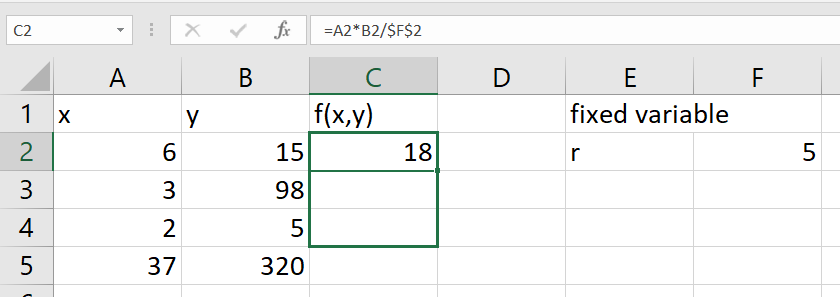
\includegraphics[width=0.8\textwidth]{Excel-tut-select-fixed}
\caption{Fixing a box value when applying a function down a column. The \$ sign before the column letter means that we are fixing the column, and the \$ sign before the row number means that we are fixing the row. One can only use one \$ sign to fix either the column or row as desired.}
\label{Fig:Excel-fixed}
\end{figure}
\item Excel also has functions that are included. Functions are called by some special command in all caps. One typically calls a function, for example the sum, as 
\begin{verbatim}
=SUM(B2:B5)
\end{verbatim}
The colon means that we take every box between B2 and B5. One could have also used that function by listing every box individually, separated by a coma. Alternatively, one could, after writing ``=SUM(", selected the boxes that one wants to be included in the function. This re-emphasizes the usefulness of arranging the data in columns.
\item Other useful functions include:
\begin{itemize}
\item \verb|=STDEV.P(x)| to calculate the standard deviation of a fluctuation population as shown in eq.~\eqref{Eq:STDev.P}.
\item \verb|=SQRT(x)| to calculate square root of $x$.
\item \verb|=Exp(x)| to calculate exponentials $e^x$.
\item \verb|PI()| to use the constant $\pi$. Note that there is no input.
\item \verb|=Sin(x)| and \verb|=Cos(x)| to calculate values in radians. The input $x$ must be in radians.
\item \verb|=AVERAGE(A2:A10)| computes the average of the boxes between A2 and A10.
\end{itemize}
There exists many other functions that could be useful.
\end{itemize}

\noindent \large \textbf{Figures} \normalsize

One can also create figures from data sets in Excel. To do so, select too columns and go into the \textbf{Insert} tab as shown in Fig.~\ref{Fig:Excel-fig-insert} to choose the type of figure that you with to display. You can choose not-adjacent columns by selecting one column, press and hold Ctrl while selecting the other column.
\begin{figure}[h]
\centering
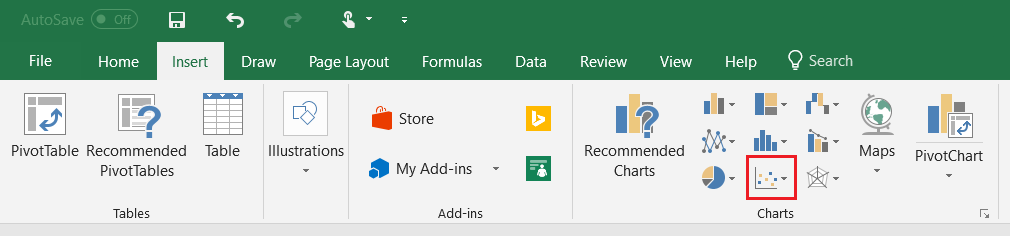
\includegraphics[width=0.8 \textwidth]{Excel-fig-insert}
\caption{Creating a plot based on some data. After selecting your data, go into the \textbf{Insert} tab and choose the type of figure that you want. The red boxed symbol is the one for scatter plots, which will most likely be your most used data display option.}
\label{Fig:Excel-fig-insert}
\end{figure}

Doing, so you should obtain something similar to Fig~\ref{Fig:Excel-fig}.
\begin{figure}[h]
\centering
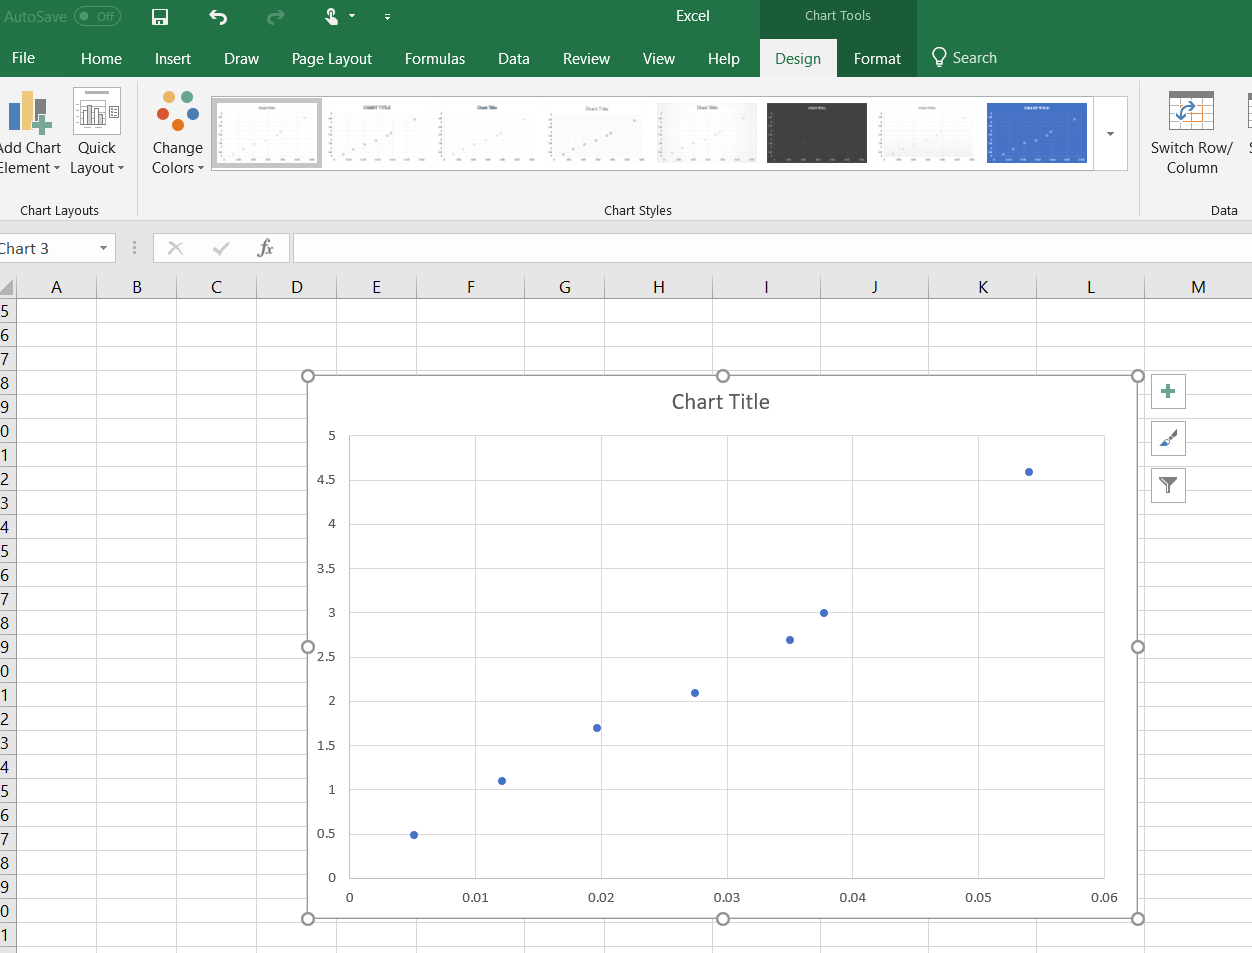
\includegraphics[width=0.8\textwidth]{Excel-fig}
\caption{Scatter plot from data}
\label{Fig:Excel-fig}
\end{figure}
From here, one can do multiple things. 
\begin{itemize}
\item By clicking the green `` + " symbol to the top right of the figure, you can add titles to your axes, error bars, a legend and a trendline.
\item By right-clicking the data points, you should see an option to ``Format Data Series". Clicking that, you will see a right bar appear, and in the ``Pain bucket" symbol, you can change the size, shape and colors of your markers.
\item By right-clicking a data point, you can add a \textbf{trendline}, in which case a right bar will also appear. Here you can choose the type of equation that you wish to fit, and if you scroll down completely, you will have the option to set an intercept, display the equation on the chart, and display the R-squared value on the chart. You can also add multiple trendlines to a single dataset to compare different fits.
\item If you right-click an empty space on the grid of the chart, you can add multiple data sets to a single chart by click ``Select Data". A pop-up window will appear with the option of renaming how your datasets will appear on the legend, and the ability to add/remove more datasets.
\item Playing around with these options, you will have the ability to change the font size of titles, colors of data points and texts, as well as change the thickness of the data points and trendlines. You can move equations, legends or other things around your chart. Don't forget that data presented must be clear.
\end{itemize}

Finally, you can add data from .txt files. To do so, go into the data tab, and in the ``Get \& Transform Data" section, there will be an option to add .txt and other types of files. Once the popup screen to import data appears, you can click on ``Edit" in the bottom right corner to have more options to manipulate your data. A useful modification is to flip your rows and columns. To do so, after clicking ``Edit", go into the ``Transform" tab in the new window, and select ``Transpose". Go back to the ``Home" tab once you are done editing your file.


\chapter{Lab Equipment}

\section{Multimeter}
A multimeter allows one to measure various electronic properties. We will be mainly interested in measuring the resistance or resistors, the capacitance of capacitors and the voltage and current of a circuit. To use the multimeter, one must attach two wires into the input and output. One can have alligator clips to attach to conducting wires more easily if necessary.

\begin{figure}[h]
\centering
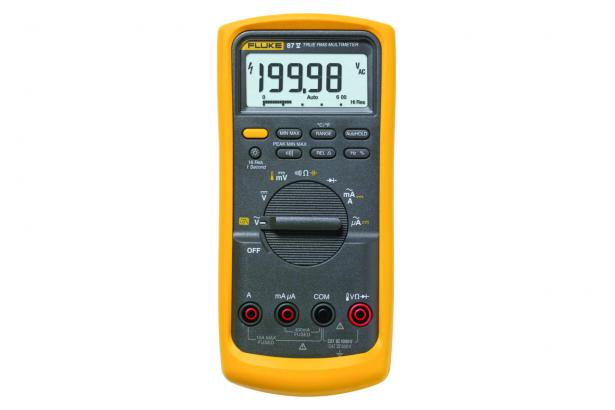
\includegraphics[width=0.7\textwidth]{appendix-DMM.png}
\label{Fig:App-DMM}
\caption{Communal DMM (model 87V Fluke). Note that you may have a different model at your individual station, but the symbols for the settings are the same. The $\Omega$ symbol (center position) allows to measure resistance. The yellow symbol with one vertical line, and another slightly curved one (next to the $\Omega$ symbol) allows to measure capacitance. You must press the yellow function button to access it.}
\end{figure}

To measure the resistance, simply take a resistor, turn the knob of the multimeter to the resistance seting ($\Omega$) and attach each wire to the two sides of a resistor. To measure the capacitance of a capacitor, simply do the same as for the resistor, but turning the knob to the capacitance setting.

To measure the voltage and current of a circuit,

\section{Arduino}
The Arduino unit requires the Arduino IDE software to run the desired scripts. Information about the Arduino code for the capacitance lab can be found \href{https://www.arduino.cc/en/Tutorial/CapacitanceMeter}{here}.

The Arduino is encased inside a utility box. The circuit diagram of it is given in Fig.\ref{Fig:App-Arduino-utility-box}.
\begin{figure}[h]
\centering
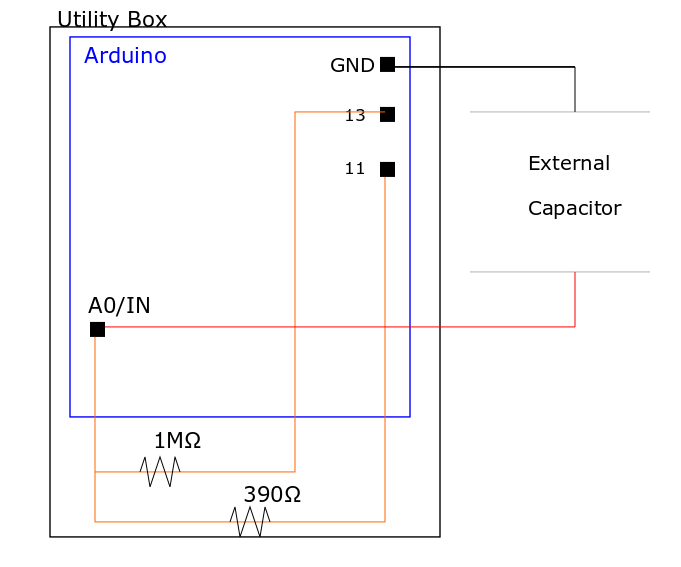
\includegraphics[width=0.6 \textwidth]{lab1-arduino-utility-box.png}
\caption{Arduino circuit inside the utility box.}
\label{Fig:App-Arduino-utility-box}
\end{figure}
The circuit consists of a 390$\Omega$ and $10^6\Omega$ resistor. The latter's value will affect the precision of the time constant measurement.
\textbf{You must input this value into the Arduino code. If you change this value, the code must reflect this change. See Fig.~\ref{Fig:ArduinoResistance}.}
\begin{figure}[h]
\centering
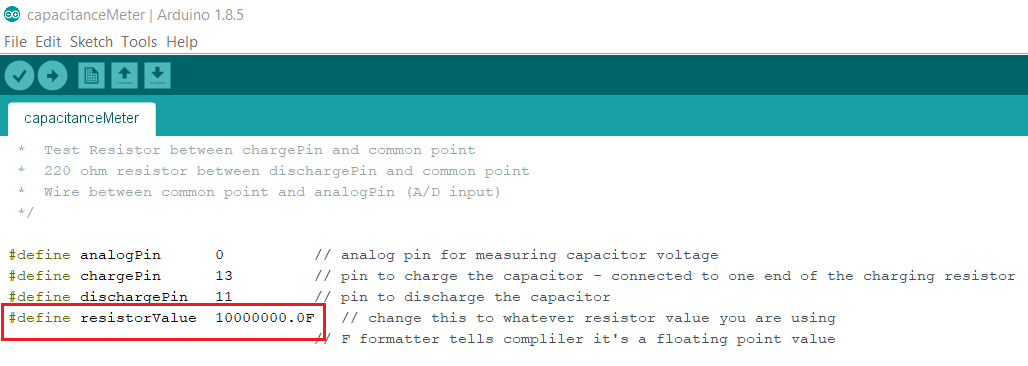
\includegraphics[width=0.9 \textwidth]{lab1-Arduino-resistance.png}
\caption{Arduino resistor value. Change the value in the red box to the resistance value of your setup. We suggest using at least $10^6 \Omega$.}
\label{Fig:ArduinoResistance}
\end{figure}

A more schematic diagram of the circuit can be found in Fig.~\ref{Fig:ArduinoSchem}.
\begin{figure}[H]
\centering
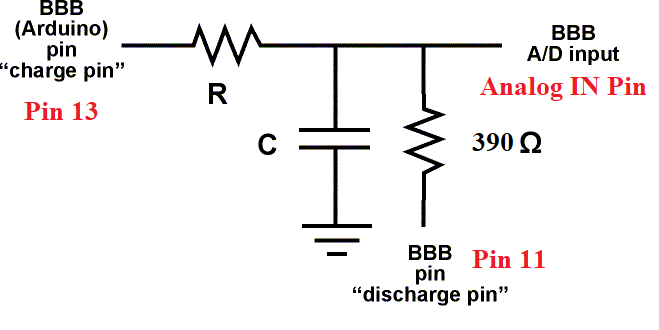
\includegraphics[scale=0.85]{CapacitanceMeterSchem.png}
\caption{Arduino ``original" circuit diagram. Note that the generic value of $R$ is fixed to $10^6\Omega$ in our case.}
\label{Fig:ArduinoSchem}
\end{figure}

\section{Reading Resistors}
\begin{figure}[h]
	\centering
	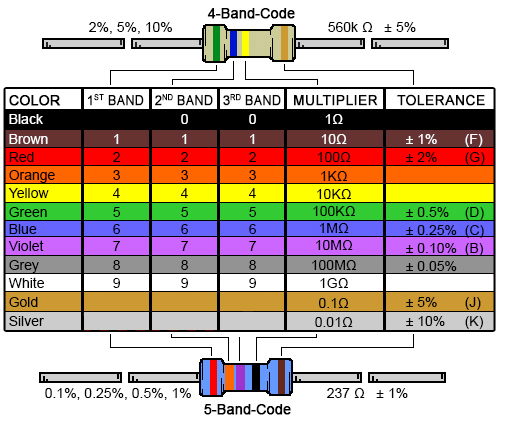
\includegraphics[scale=1.0]{appendix-resistor-chart.png}
	\caption{Resistor color chart.}
	\label{Fig:resistor-chart}
\end{figure}

The color code for resistors changes according to where the position (or number) of the band is in the resistor, starting from where there is a greater number of bands. In the above image this is from left to right. As a rule, the last two bands correspond to the multiplier and tolerance respectively, while the rest correspond to the ohmic value. For example, as shown in the figure, for the 4-Band-Code resistor we have: Green (5) and Blue (6), times 10 K$\Omega$ (Yellow) with a tolerance of $\pm$ 5\% (Gold) so that resistor is 560 ($\pm$ 5\%)  K$\Omega$. For the 5-Band-Code resistor we have: Red (2), Orange (3) and Purple(7), times 1 $\Omega$ (Black) with a tolerance of  $\pm$ 1\%(Brown) that is a resistor of 237 $\pm$1\% $\Omega$.

\section{Bread Boards}
In Lab 2, you will use a bread board similar to that of Fig.~\ref{Fig:lab2-bread-board} to connect your RC circuit.
\begin{figure}[h]
\centering
\includegraphics[scale=0.06]{lab2-bread-board}
\caption{A typical bread board used in Lab 2.}
\label{Fig:lab2-bread-board}
\end{figure}

In the middle section of the bread board, there are metallic strips for every row (see for example the green strips for rows 25-27 in the figure).
On the side, there vertical strips as shown for the red ``+" column on the right.
You may have another type of bread board, but the design remains the same: you will have a section where metallic strips are distributed horizontally,
and another one where the strips are laid out vertically.



\section{IOLab}
Here are additional comments about the functionality of the IOLab

\begin{itemize}
\item You can zoom in and out
\item How to get STD and mean
\item How to load previous datasets
\end{itemize}

\section{Oscilloscope}
In lab 3, we will use a digital oscilloscope. An oscilloscope is a valuable tool often used in many applications. Its most important function is the
ability to measure voltages that vary in time. The oscilloscope allows us to ``visualize" how this
voltage changes. To fully characterize a voltage that varies in time using a hand-held voltmeter,
you would have to plot how the readings change with time on a graph. This is not only time
consuming, but impossible to do if the voltage changes too rapidly (for example, the voltage
from a wall socket changes sinusoidally from +115 V to -115 V and back to +115 V in 1/60th of
a second). To understand the principle behind an oscilloscope we will explain how an analog cathode ray oscilloscope (CRO) works. The CRO report voltage by tracking the vertical position of an electron beam rapidly
sticking a fluorescent screen as it exists the space between two charged parallel conducting
plates as is illustrated in Fig.~\ref{Fig:Appendix-CRO-data}. It plots the voltage on a screen along a vertical axis, and can
also track changes of this voltage in time (horizontal axis) in a fraction of a microsecond.

%\cesar{Add instructions on how to use the oscilloscope.}

\begin{figure}[h]
\centering
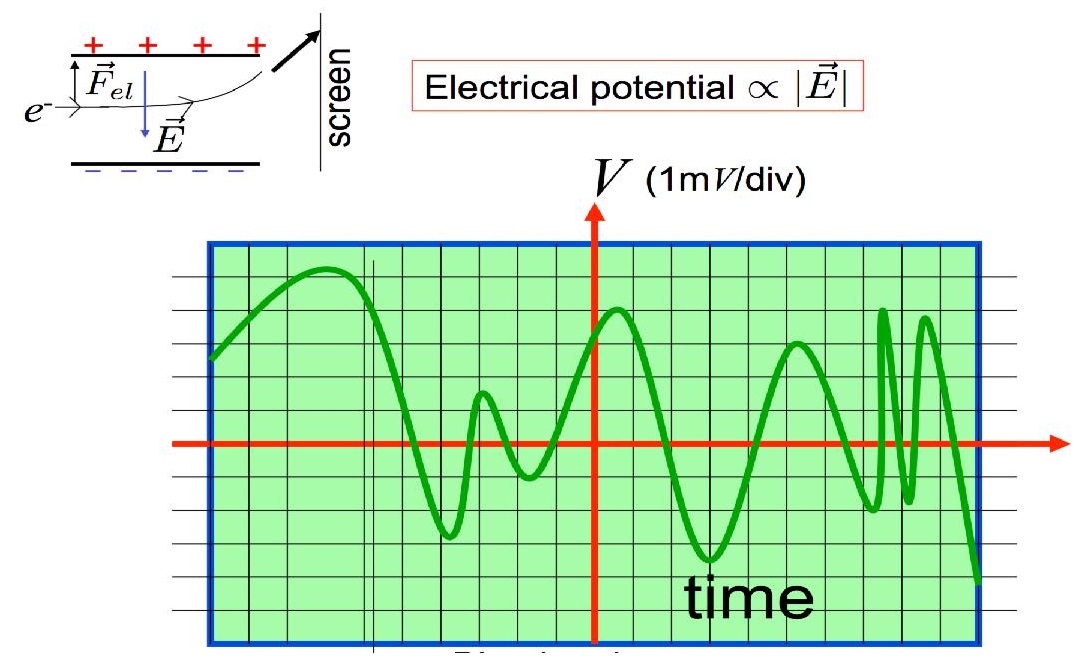
\includegraphics[scale=1.2]{appendix-cro-data}
\caption{Operation of a CRO}
\label{Fig:Appendix-CRO-data}
\end{figure}

To use the oscilloscope you must first plug it into an outlet, turn it on by clicking the 'run/stop' button glowing green, and then plug in your BNC cable into the connection labeled Channel A - shown in red in Figure \ref{Fig:Appendix-Osc}. You must then adjust the position and scale knobs, shown in green until you see a signal on the screen. The vertical position knob on the left will adjust the $y$ position of the signal on the screen. The scale knob on the other hand, will modify the value in volts and time in \textit{y} and \textit{x} respectively of each of the squares or divisions on the screen. Explained in another manner these knobs allow you to control the zoom (or scale) in/out in each direction separately. You can also use the button labeled cursor, shown in orange, to adjust the cursor on the screen to aid you in measuring the frequency or voltage of the signal. The oscilloscope has other options such as DC or AC coupling that will already be set up for you. It will not be necessary to play around with any of the other options during the lab. 

%To use the oscilloscope you must first plug it into an outlet, turn it on, and then plug in your positive and negative electrodes into the connection labeled Channel A shown in orange in Figure \ref{Fig:Appendix-CRO}. You must then adjust the position, volts/div (12), and time/div (13) knobs until you see a signal on the screen (19). The position knob will adjust the vertical position of the signal. The volts/div and time/div on the other hand, will modifiy the value in volts and time and in \textit{y} and \textit{x} respectively of each of the squares or divisions. Explained in another manner these knobs allow you to control the zoom in/out in each direction separetely. The oscilloscope has other options such as DC or AC coupling that will already be set up for you. It will not be necessary to play around with any of the other options during the lab. 

%\begin{figure}[h]
%\centering
%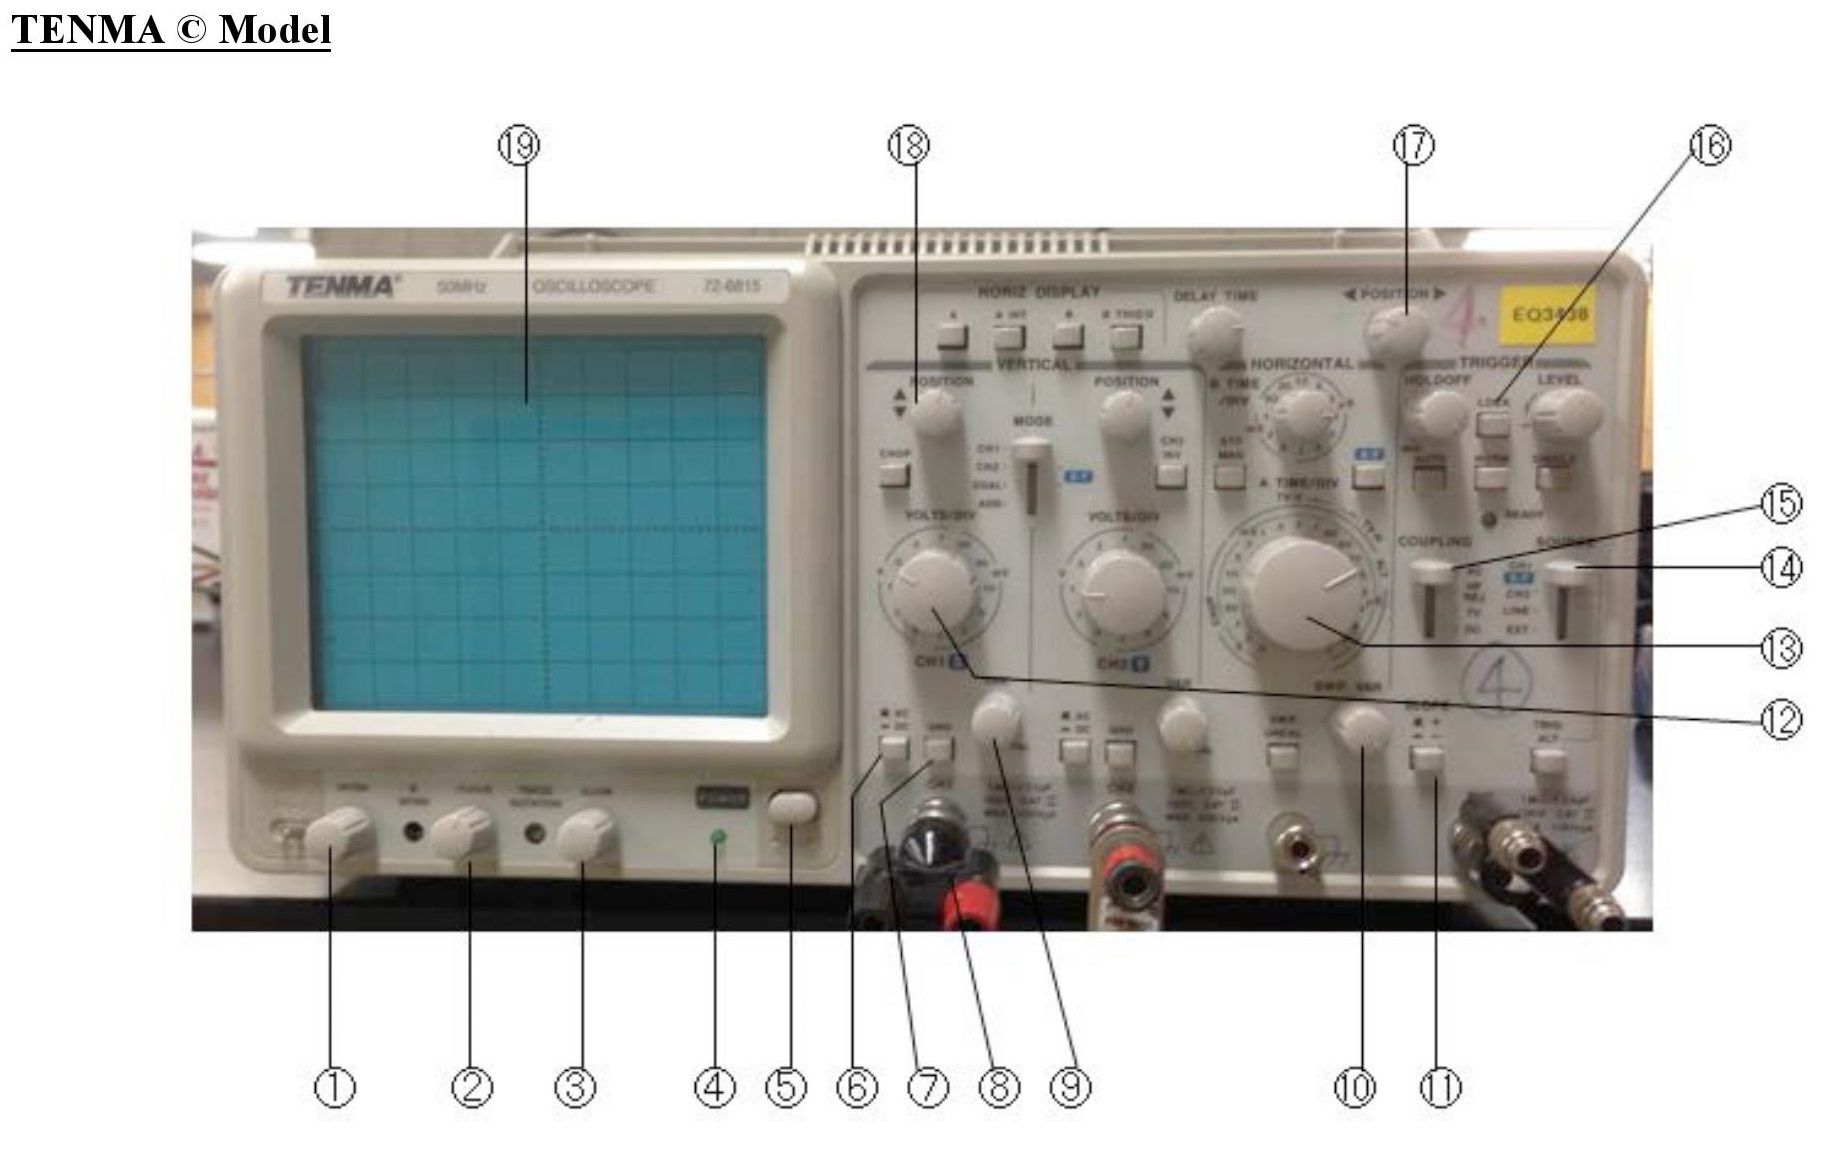
\includegraphics[scale=1]{appendix-cro-pic}
%\caption{Photograph of one CRO model}
%\label{Fig:Appendix-CRO}
%\end{figure}

\begin{figure}[h]
	\centering
	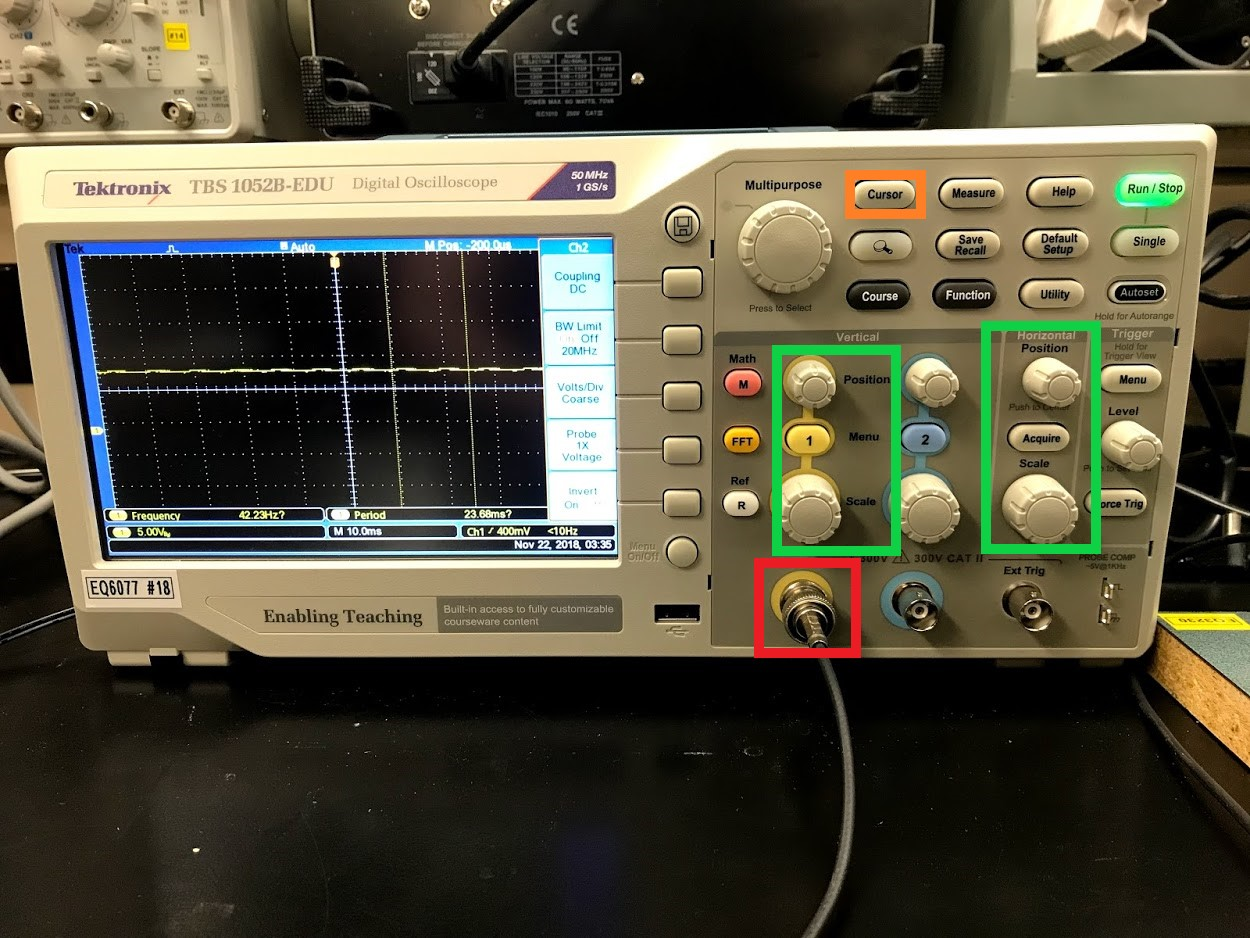
\includegraphics[scale=0.5]{appendix-digosc-label-pic.jpg}
	\caption{Photograph of a digital model}
	\label{Fig:Appendix-Osc}
\end{figure}

\chapter{More about statistics} \label{App:R2}

\noindent \large \textbf{Coefficient of determination} \normalsize

To determine the precision of a fit, one can look at its $R^2$ value, also known as the \textit{coefficient of determination}. Consider a dataset of $N$ datapoints with values $y_i$, $i$ going from $1$ to $N$. We define the \textit{total sum of squares} as
\begin{equation}
SS_{tot} = \displaystyle \sum_{i=1}^N (y_i - \bar{y})^2 = (y_1 - \bar{y})^2 + (y_2 - \bar{y})^2 + ... (y_N - \bar{y})^2.
\end{equation}
This is a measure of how your dataset differs from its average.

Now consider the values $f_i$ of a fit, where $i$ are the values of the fit corresponding to $x_i$ of $y_i$ value. We can also define the \textit{residual sum of squares} which is a measure of how your fit differs from your fit. This is given as
\begin{equation}
SS_{res} = \displaystyle \sum_{i=1}^{N} (y_i - f_i)^2 = (y_1 - f_1)^2 + (y_2 - f_2)^2 + ... (y_N - f_N)^2.
\end{equation}

Finally, given the results above, we can define the \textit{coefficient of determination} as
\begin{equation}
R^2 = 1 - \frac{SS_{res}}{SS_{tot}}
\end{equation}
which is a ratio of how your data fluctuations with respect to how you data differs from its fit. A good coefficient of determination is $R^2=1$. This can be computed automatically in Excel.


\end{appendix}

%\bibliographystyle{naturemag}
%\bibliography{references}

\end{document}